%% !TeX program = lualatex

%\listfiles	
% **************************
% STOP - Bitte zuerst lesen, bevor Sie weitermachen
%
% Einige Dinge müssen Sie an Ihre Bedürfnisse (und die Vorgaben Ihres
% Betreuers anpassen. Editieren Sie dazu die Datei docinfo.tex).
%
% 1. Sprache
% Das Template unterstützt Deutsch und Englisch, Standard ist Deutsch.
% Wenn Sie Englisch verwenden wollen, ändern Sie bitte direkt am Anfang
% dieser Datei den Eintrag
%    \newcommand{\hsmasprache}{de}
% auf
%    \newcommand{\hsmasprache}{en}
%
% 2. Form der Abgabe
% Das Template unterstützt sowohl eine digitale Abgabe, als auch eine Abgabe
% auf Papier. Bei einer Papierabgabe wird ein doppelseitiger Druck vorbereitet
% und der Titel wird so platziert, dass er in das Fenster des offiziellen
% Umschlages der Hochschule passt.
% Bei einer digitalen Abgabe (als PDF) wird der Titel zentriert und als
% Format wird einseitig gewählt. Außerdem wird die Datei unterschrift.png
% auf dem Blatt mit der Erklärung zur Eigenständigkeit eingebunden.
%
% 3. Zitierstil
% Abhängig von dem gewünschten Zitierstil passen Sie bitte in
% hma.cls die Einstellungen bei \RequirePackage[backend=biber...
% an. Wie ist dort genau erklärt.
% Achtung: Wenn Sie als Zitierstil Fußnoten wählen bzw. generell
% -------  mit Fußnoten arbeiten, dann beachten Sie bitte, dass
%          Fußnoten in Bildunterschriften und Tabellenüberschriften
%          nicht funktionieren.
%          Siehe hierzu https://texfaq.org/FAQ-ftncapt
%          und https://texfaq.org/FAQ-footintab
%          Sinnvollerweise verzichten Sie auf Fußnoten an diesen
%          Stellen und fügen Quellen einfach per \parancite ein.
%
% 4. Doppelseitiger oder einseitiger Druck
% Das Template bestimmt, ob einseitig oder doppelseitig gedruckt wird
% anhand der Abgabeform (papier / digital). Wollen sie dies übersteuern,
% müssen Sie in der Datei preambel.tex folgende Zeile
% \KOMAoptions{twoside=true} für doppelsetigen Druck
% \KOMAoptions{twoside=false} für einsetigen Druck
% direkt vor \usepackage{xcolor} einsetzen. Prinzipiell sollten Sie aber
% das vorgeschlagene Format einfach so lassen.
%
% 5. Unnötige Teile entfernen
% Entfernen Sie die Teile, die Sie nicht brauchen, z.B. Anhänge
%
% 6. Silbentrennung
% LaTeX führt eine automatische Silbentrennung durch. Allerdings
% werden Wörter, die bereits einen Bindestrich enthalten nicht
% getrennt, z.B. Datenschutz-Grundverordnung. Wenn Sie Ihren Text auf
% Deutsch schreiben, können Sie dann alternativ "= für den Bindestrich
% im Wort verwenden, z.B. Datenschutz"=Grundverordnung, damit LaTeX
% weiterhin richtig trennt.
% Ist die Silbentrennung aus einem anderen Grund nicht erfolgt, sodass
% das Wort über den rechten Rand hinaussteht oder wenn Sie eine weitere
% Trennstelle wollen, können Sie LaTeX helfen, indem Sie weitere
% Trennstellen angeben. Dies geschieht durch "- als Zeichen, z.B.
% Staats"-vertrag.
%
% 7. Nummerierung der Fußnoten
% LaTeX beginnt die Nummerierung der Fußnoten in jedem Kapitel wieder
% bei 1. In diesem Template wird die fortlaufende Nummerierung der Fußnoten 
% über die gesamte Arbeit umgesetzt.  
%
% 8. Unterschrift
% Bei einer Abgabe auf Papier unterschreiben Sie die Arbeit eigenhändig.
% Geben Sie allerdings digital ab, sollten Sie die Datei unterschrift.png in dem 
% Ordner /bilder durch einen Scan Ihrer eigenen Unteschrift ersetzen - andernfalls
% unterschreiben Sie als Max Mustermann ;-)
% *******************************************************************

% Dokumenteneinstellungen und Infos importieren
% -------------------------------------------------------
% Daten für die Arbeit
% Wenn hier alles korrekt eingetragen wurde, wird das Titelblatt
% automatisch generiert. D.h. die Datei titelblatt.tex muss nicht mehr
% angepasst werden.

% Titel der Arbeit auf Deutsch
\newcommand{\hsmatitelde}{Einsatz eines Flux-Kompensators für Zeitreisen mit einer maximalen Höchstgeschwindigkeit von WARP~7}

% Titel der Arbeit auf Englisch
\newcommand{\hsmatitelen}{Application of a flux compensator for timetravel with a maximum velocity of warp~7}

% Weitere Informationen zur Arbeit
\newcommand{\hsmaort}{Mannheim}    % Ort
\newcommand{\hsmaautorvname}{Max} % Vorname(n)
\newcommand{\hsmaautornname}{Mustermann} % Nachname(n)
\newcommand{\hsmadatum}{25.02.2019} % Datum der Abgabe
\newcommand{\hsmajahr}{2019} % Jahr der Abgabe
\newcommand{\hsmafirma}{Paukenschlag GmbH, Mannheim} % Firma bei der die Arbeit durchgeführt wurde
\newcommand{\hsmabetreuer}{Prof. Peter Mustermann, Hochschule Mannheim} % Betreuer an der Hochschule
\newcommand{\hsmazweitkorrektor}{Erika Mustermann, Paukenschlag GmbH} % Betreuer im Unternehmen oder Zweitkorrektor
\newcommand{\hsmafakultaet}{I} % I für Informatik oder E, S, B, D, M, N, W, V
\newcommand{\hsmastudiengang}{IB} % IB IMB UIB CSB IM MTB (weitere siehe titleblatt.tex)

% Zustimmung zur Veröffentlichung
\setboolean{hsmapublizieren}{true}   % Einer Veröffentlichung wird zugestimmt
\setboolean{hsmasperrvermerk}{false} % Die Arbeit hat keinen Sperrvermerk

% -------------------------------------------------------
% Abstract

% Kurze (maximal halbseitige) Beschreibung, worum es in der Arbeit geht auf Deutsch
\newcommand{\hsmaabstractde}{Jemand musste Josef K. verleumdet haben, denn ohne dass er etwas Böses getan hätte, wurde er eines Morgens verhaftet. Wie ein Hund! sagte er, es war, als sollte die Scham ihn überleben. Als Gregor Samsa eines Morgens aus unruhigen Träumen erwachte, fand er sich in seinem Bett zu einem ungeheueren Ungeziefer verwandelt. Und es war ihnen wie eine Bestätigung ihrer neuen Träume und guten Absichten, als am Ziele ihrer Fahrt die Tochter als erste sich erhob und ihren jungen Körper dehnte. Es ist ein eigentümlicher Apparat, sagte der Offizier zu dem Forschungsreisenden und überblickte mit einem gewissermaßen bewundernden Blick den ihm doch wohl bekannten Apparat. Sie hätten noch ins Boot springen können, aber der Reisende hob ein schweres, geknotetes Tau vom Boden, drohte ihnen damit und hielt sie dadurch von dem Sprunge ab. In den letzten Jahrzehnten ist das Interesse an Künstlern sehr zurückgegangen. Aber sie überwanden sich, umdrängten den Käfig und wollten sich gar nicht fortrühren.}

% Kurze (maximal halbseitige) Beschreibung, worum es in der Arbeit geht auf Englisch
\newcommand{\hsmaabstracten}{The European languages are members of the same family. Their separate existence is a myth. For science, music, sport, etc, Europe uses the same vocabulary. The languages only differ in their grammar, their pronunciation and their most common words. Everyone realizes why a new common language would be desirable: one could refuse to pay expensive translators. To achieve this, it would be necessary to have uniform grammar, pronunciation and more common words. If several languages coalesce, the grammar of the resulting language is more simple and regular than that of the individual languages. The new common language will be more simple and regular than the existing European languages. It will be as simple as Occidental; in fact, it will be Occidental. To an English person, it will seem like simplified English, as a skeptical Cambridge friend of mine told me what Occidental is.}


% Preambel importieren
% Document type and used packages
\documentclass[open=right, % Kapitel darf nur auf rechten Seite beginnen
    paper=A4,               % DIN-A4-Papier
    a4paper,                % DIN-A4-Papier
    12pt,                   % Schriftgöße
    headings=small,         % Kleine Überschriften
    headsepline=true,       % Trennlinie am Kopf der Seite
    footsepline=false,      % Trennlinie am Fuß der Seite
    bibliography=totoc,     % Literaturverzeichnis in das Inhaltsverzeichnis aufnehmen
    twoside=on,             % Doppelseitiger Druck - auf off stellen für einseitig
    DIV=7,
    chapterprefix=true,     % Kapitel x vor dem Kapitelnamen
    cleardoublepage=plain]{scrbook} 

\usepackage{scrpage2}

% Pakete einbinden, die benötigt werden
\usepackage[utf8]{inputenc}       % Dateien in UTF-8 benutzen
\usepackage[T1]{fontenc}          % Zeichenkodierung
\usepackage{graphicx}             % Bilder einbinden
\usepackage[ngerman,english]{babel}       % Deutsch und Englisch unterstützen
\usepackage{xcolor}               % Color support
\usepackage{amsmath}              % Matheamtische Formeln
\usepackage{amsfonts}             % Mathematische Zeichensätze
\usepackage{amssymb}              % Mathematische Symbole
\usepackage{float}                % Fließende Objekte (Tabellen, Grafiken etc.)
\usepackage{booktabs}             % Korrekter Tabellensatz
\usepackage[printonlyused]{acronym}   % Abkürzungsverzeichnis [nur verwendete Abkürzugen]
\usepackage{makeidx}              % Sachregister
\usepackage{listings}             % Source Code listings
\usepackage{listingsutf8}         % Listings in UTF8
\usepackage[hang,font={sf,footnotesize},labelfont={footnotesize,bf}]{caption} % Beschriftungen
\usepackage[scaled]{helvet}       % Schrift Helvetia laden
\usepackage[absolute]{textpos}	  % Absolute Textpositionen (für Deckblatt)
\usepackage{calc}                 % Berechnung von Positionen
\usepackage{blindtext}            % Blindtexte
\usepackage[bottom=40mm,left=35mm,right=35mm,top=30mm]{geometry} % Ränder ändern
\usepackage[square]{natbib}       % Literaturverzeichnis nach DIN mit eckigen Klammern bei \citep
\usepackage{setspace}             % Abstände korrigieren
\usepackage{ifthen}               % Logische Bedingungen mit ifthenelse
\usepackage{scrhack}              % Get rid of tocbasic warnings
\usepackage[pagebackref=false]{hyperref}  % Hyperlinks
\usepackage[all]{hypcap}          % Korrekte Verlinkung von Floats

% Farben definieren
\definecolor{linkblue}{RGB}{0, 0, 100}
\definecolor{linkblack}{RGB}{0, 0, 0}
\definecolor{comment}{RGB}{63, 127, 95}
\definecolor{darkgreen}{RGB}{14, 144, 102}
\definecolor{darkblue}{RGB}{0,0,168}
\definecolor{darkred}{RGB}{128,0,0}
\definecolor{javadoccomment}{RGB}{0,0,240}

% Einstellungen für das Hyperlink-Paket
\hypersetup{
    colorlinks=true,      % Farbige links verwenden       
%    allcolors=linkblue,
    linktoc=all,          % Links im Inhaltsverzeichnis
    linkcolor=linkblack,  % Querverweise
    citecolor=linkblack,  % Literaturangaben
	filecolor=linkblack,  % Dateilinks
	urlcolor	=linkblack    % URLs
}

% Einstellungen für Quelltexte
\lstset{     
      xleftmargin=0.2cm,     
      basicstyle=\footnotesize\ttfamily,
      keywordstyle=\color{darkgreen},
      identifierstyle=\color{darkblue},
      commentstyle=\color{comment}, 
      stringstyle=\color{darkred}, 
      tabsize=2,
      lineskip={2pt},
      columns=flexible,
      inputencoding=utf8,
      captionpos=b,
      breakautoindent=true,
	  breakindent=2em,
	  breaklines=true,
	  prebreak=,
	  postbreak=,
      numbers=none,
      numberstyle=\tiny,
      showspaces=false,      % Keine Leerzeichensymbole
      showtabs=false,        % Keine Tabsymbole
      showstringspaces=false,% Leerzeichen in Strings
      morecomment=[s][\color{javadoccomment}]{/**}{*/},
      literate={Ö}{{\"O}}1 {Ä}{{\"A}}1 {Ü}{{\"U}}1 {ß}{{\ss}}2 {ü}{{\"u}}1 {ä}{{\"a}}1 {ö}{{\"o}}1
}

\urlstyle{same}

% Einstellungen für Überschriften
\renewcommand*{\chapterformat}{%
  \Large\chapapp~\thechapter   % Große Schrift
  \vspace{0.3cm}               % Abstand zum Titel des Kapitels
}

% Abstände für die Überschriften setzen
\renewcommand{\chapterheadstartvskip}{\vspace*{2.6cm}}
\renewcommand{\chapterheadendvskip}{\vspace*{1.5cm}}

\RedeclareSectionCommand[
  beforeskip=-1.8\baselineskip,
  afterskip=0.25\baselineskip]{section}

\RedeclareSectionCommand[
  beforeskip=-1.8\baselineskip,
  afterskip=0.15\baselineskip]{subsection}


% In der Kopfzeile nur die kurze Kapitelbezeichnung (ohne Kapitel davor)
\renewcommand*\chaptermarkformat{\thechapter\autodot\enskip}
\automark[chapter]{chapter}

% Einstellungen für Schriftarten
\setkomafont{pagehead}{\normalfont\sffamily}
\setkomafont{pagenumber}{\normalfont\sffamily}
\setkomafont{paragraph}{\sffamily\bfseries\small}
\setkomafont{subsubsection}{\sffamily\itshape\bfseries\small}
\addtokomafont{footnote}{\footnotesize}
\setkomafont{chapter}{\LARGE\selectfont\bfseries}

% Wichtige Abstände
\setlength{\parskip}{0.2cm}  % 2mm Abstand zwischen zwei Absätzen
\setlength{\parindent}{0mm}  % Absätze nicht einziehen
\clubpenalty = 10000         % Keine "Schusterjungen"
\widowpenalty = 10000        % Keine "Hurenkinder"
\displaywidowpenalty = 10000 % Keine "Hurenkinder"
\renewcommand{\footnotesize}{\fontsize{9}{10}\selectfont} % Größe der Fußnoten
\setlength{\footnotesep}{8pt} % Abstand zwischen den Fußnoten

% Index erzeugen
\makeindex

% Einfacher Font-Wechsel über dieses Makro
\newcommand{\changefont}[3]{
\fontfamily{#1} \fontseries{#2} \fontshape{#3} \selectfont}

% Eigenes Makro für Bilder
\newcommand{\bild}[3]{
\begin{figure}[h]
  \centering
  \includegraphics[width=#2]{#1}
  \caption{#3}
  \label{#1}
\end{figure}}

% Wo liegt Sourcecode?
\newcommand{\srcloc}{src/}

% Wo sind die Bilder?
\graphicspath{{bilder/}}

% Makros für typographisch korrekte Abkürzungen
\newcommand{\zb}[0]{z.\,B.\ }
\newcommand{\dahe}[0]{d.\,h.\ }
\newcommand{\ua}[0]{u.\,a.\ }

% Flags für Veröffentlichung und Sperrvermerk
\newboolean{hsmapublizieren}
\newboolean{hsmasperrvermerk}



%Abstrakt Ihrer Abschlussarbeit 
% -------------------------------------------------------
% Abstrakt / Abstract
% Achtung: Wenn Sie im Abstrakt Anführungszeichen verwenden wollen, dann benutzen Sie
%          nicht "` und "', sondern \enquote{}. "` und "' werden nicht richtig
%          erkannt.

% Kurze (maximal halbseitige) Beschreibung, worum es in der Arbeit geht auf Deutsch
\newcommand{\hsmaabstractde}{Die Arbeit handelt von Entscheidungssystemen der Game-AI. Entscheidungssysteme dienen der Entscheidungsfindung von Non-Player Charactern (NPC) in Videospielen und dienen der Immersion. Dabei werden die Entscheidungssysteme Finite State Machine (FSM), Behavior Tree (BT) und Goal oriented Action Planning (GOAP) erklärt, miteinander verglichen und anschließend bewertet. Im Fokus liegen das Entscheidungssystem GOAP, zu dem im Vergleich zu anderen Entscheidungssystemen wenige Bibliotheken und Dokumentationen existieren. Eine Bewertung der drei Enscheidungssystemen wird dem Entwickler die Wahl dieser erleichtern. Für den Vergleich werden die Entscheidungssysteme in ein Videospiel implementiert. Aus der gewonnen Erfahrung, Benchmarks und wissenschaftlicher Literatur werden diese abschließend bewertet. Die FSM wird dabei für einfache, der BT für mittlere bis komplexe und GOAP für komplexe NPC-Verhalten empfohlen.}

% Kurze (maximal halbseitige) Beschreibung, worum es in der Arbeit geht auf Englisch
\newcommand{\hsmaabstracten}{The thesis focuses on decision-making systems in Game AI. These systems are responsible for the decision-making of Non-Player Characters (NPCs) in video games and contribute to immersion. The decision-making systems Finite State Machine (FSM), Behavior Tree (BT), and Goal-Oriented Action Planning (GOAP) are explained, compared, and evaluated. The primary focus is on GOAP, as there are fewer libraries and less documentation available for it compared to other decision-making systems. Evaluating these three systems will help developers make an informed choice. For the comparison, the decision-making systems are implemented in a video game. Based on the gained experience, benchmarks, and scientific literature, they are assessed in detail. The FSM is recommended for simple behaviors, BT for medium to complex behaviors, and GOAP for complex NPC behaviors.}



% Literatur-Datenbank
\addbibresource{literatur.bib}   % BibLaTeX-Datei mit Literaturquellen einbinden


% Anfang des Dokuments
\begin{document}	


%Laden der Dateien mit Abkürzungen, Begriffserklärungen (Glossar), Symbole
% Tragen Sie hier alle Abkürzungen ein, die in der Arbeit benutzt werden

makeindex -s %.ist -t %.alg -o %.acr %.acn

\newacronym{abk}{ABK}{Abkürzung}
\newacronym{acm}{ACM}{Association of Computing Machinery}
\newacronym{pdf}{PDF}{Portable Document Format}
\newacronym{ieee}{IEEE}{Institute of Electrical and Electronics Engineers}
\newacronym{iso}{ISO}{International Organization for Standardization}
\newacronym[plural=ISPs,firstplural=Internet Service Providers (ISPs)]{isp}{ISP}{Internet Service Provider}
\newacronym{doi}{DOI}{Digital Object Identifier}

% Glossareinträge
\newglossaryentry{glos:amplification}{name={Amplification}, description={describes the disproportionate increase of a response packet compart to the initial request packet.}}

\newglossaryentry{symb:Pi}{name=\ensuremath{\pi},
	description={Geometrical value},
	unit={},
	type=symbolslist}



\newglossaryentry{symb:energyconsump}{name=\ensuremath{P},
	description={Energy consumption},
	unit={\si{kW}},
	type=symbolslist}
	
	
\pagestyle{headings}
\tableofcontents


\mainmatter

%% Ihre Inhaltsdateien werden an dieser Stelle in das Dokument eingefügt
%\chapter{Schreibstil}

\section{Fremdsprachige Begriffe}

Wenn Sie Ihre Arbeit auf Deutsch verfassen, gehen Sie sparsam mit englischen Ausdrücken um. Natürlich brauchen Sie etablierte englische Fachbegriffe, wie z.\,B. \textit{Interrupt}, nicht zu übersetzen. Sie sollten aber immer dann, wenn es einen gleichwertigen deutschen Begriff gibt, diesem den Vorrang geben. Den englischen Begriff (\textit{term}) können Sie dann in Klammern oder in einer Fußnote\footnote{Englisch: \textit{footnote}.} erwähnen. Absolut unakzeptabel sind deutsch gebeugte englische Wörter oder Kompositionen aus deutschen und englischen Wörtern wie z.\,B. downgeloadet, upgedated, Keydruck oder Beautyzentrum.


\section{Zitate}

\subsection{Zitate im Text}

Wichtig ist das korrekte Zitieren von Quellen, wie es auch von \cite{Kornmeier2011} dargelegt wird. Interessant ist in diesem Zusammenhang auch der Artikel von \cite{Kramer2009}. Häufig werden die Zitate auch in Klammern gesetzt, wie bei \parencite{Kornmeier2011} und mit Seitenzahlen versehen \parencite[S. 22--24]{Kornmeier2011}.

Bei Webseiten wird auch die URL und das Abrufdatum mit angegeben \parencite{Gao2017}. Wenn die URL nicht korrekt umgebrochen wird, lohnt es sich, an den Parametern \textit{biburl*penalty} in der \texttt{preambel.tex} zu drehen. Kleinere Werte erhöhen die Wahrscheinlichkeit, dass getrennt wird.

\subsection{Zitierstile}

Verwenden Sie eine einheitliche und im gesamten Dokument konsequent durchgehaltene Zitierweise\index{Zitierweise}. Es gibt eine ganze Reihe von unterschiedlichen Standards für das Zitieren und den Aufbau eines Literaturverzeichnisses. Sie können entweder mit Fußnoten oder Kurzbelegen im Text arbeiten. Welches Verfahren Sie einsetzen ist Ihnen überlassen, nur müssen Sie es konsequent durchhalten.

In der Informatik ist das Zitieren mit Kurzbelegen\index{Zitat!Kurzbeleg} im Text (Harvard"=Zitierweise) weit verbreitet, wobei für das Literaturverzeichnis häufig die Regeln der \acs{ACM} oder \acs{IEEE} angewandt werden.\footnote{Einen Überblick über viele verschiedene Zitierweisen finden Sie in der \url{http://amath.colorado.edu/documentation/LaTeX/reference/faq/bibstyles.pdf}}

Am einfachsten ist es, wenn Sie das \verb+\autocite{}+-Kommando verwenden. Bei diesem Kommando können Sie in der Datei \texttt{perambel.tex} festlegen, wie die Zitate generell aussehen sollen, \zb \ ob sie in Fußnoten erfolgen sollen oder nicht. Wollen Sie von dem globalen Zitierstil abweichen, können Sie weiterhin spezielle Kommandos benutzen:

\begin{itemize}
	\item \verb+\autocite{Willberg1999}+: \autocite{Willberg1999}
	\item \verb+\cite{Willberg1999}+: \cite{Willberg1999}
	\item \verb+\parencite{Willberg1999}+: \parencite{Willberg1999}
	\item \verb+\footcite{Willberg1999}+: \footcite{Willberg1999}
	\item \verb+\citeauthor{Willberg1999}+: \citeauthor{Willberg1999}
	\item \verb+\citeauthor*{Willberg1999}+: \citeauthor*{Willberg1999}
	\item \verb+\citetitle{Willberg1999}+: \citetitle{Willberg1999}
	\item \verb+\fullcite{Willberg1999}+: \fullcite{Willberg1999}
\end{itemize}

Denken Sie daran, dass das Übernehmen einer fremden Textstelle ohne entsprechenden Hinweis auf die Herkunft in wissenschaftlichen Arbeiten nicht akzeptabel ist und dazu führen kann, dass die Arbeit nicht anerkannt wird. Plagiate\index{Plagiat!Bewertung} werden mit mangelhaft (5,0) bewertet und können weitere rechtliche Schritte nach sich ziehen.


\subsection{Zitieren von Internetquellen}

Internetquellen\index{Zitat!Internetquellen} sind normalerweise \textit{nicht} zitierfähig. Zum einen, weil sie nicht dauerhaft zur Verfügung stehen und damit für den Leser möglicherweise nicht beschaffbar sind und zum anderen, weil häufig der wissenschaftliche Anspruch fehlt.\footnote{Eine lesenswerte Abhandlung zu diesem Thema findet sich (im Internet) bei \cite{Weber2006}}

Wenn ausnahmsweise doch eine Internetquelle zitiert werden muss, z.\,B. weil für eine Arbeit dort Informationen zu einem beschriebenen Unternehmen abgerufen wurden, sind folgende Punkte zu beachten:

\begin{itemize}
\item Die Webseite ist auszudrucken und im Anhang der Arbeit beizufügen,
\item das Datum des Abrufs und die URL sind anzugeben,
\item verwenden Sie Internet"=Seiten ausschließlich zu illustrativen Zwecken (z.\,B. um einen Sachverhalt noch etwas genauer zu erläutern), aber nicht zur Faktenvermittlung (z.\,B. um eine Ihrer Thesen zu belegen).
\end{itemize}

Wenn Sie aufgrund der Natur Ihrer Arbeit sehr viele Internetquellen benötigen, dann können Sie diese statt sie auszudrucken auch in elektronischer Form abgeben (CD/DVD). Als Abgabeformat der elektronischen Quellen ist PDF/A\footnote{Bei PDF/A handelt es sich um ein besonders stabile Variante des \ac{PDF}, die von der  \ac{ISO} standardisiert wurde.} vorteilhaft, weil es von allen Formaten die größte Stabilität besitzt.
Auf der CD/DVD geben Sie bitte auch eine HTML"=Version des Literaturverzeichnisses ab, in der die Online"=Quellen sowie die gespeicherten PDF"=Dateien verlinkt sind.

Wikipedia\index{Zitat!Wikipedia} stellt einen immensen Wissensfundus dar und enthält zu vielen Themen hervorragende Artikel. Sie müssen sich aber darüber im Klaren sein, dass die Artikel in Wikipedia einem ständigen Wandel unterworfen sind und nicht als Quelle für wissenschaftliche Fakten genutzt werden sollten. Es gelten die allgemeinen Regeln für das Zitieren von Internetquellen. Sollten Sie doch Wikipedia nutzen müssen, verwenden Sie bitte ausschließlich den Perma"=Link\footnote{Sie erhalten den Permalink über die Historie der Seite und einen Klick auf das Datum.}\index{Permalink} zu der Version der Seite, die Sie aufgerufen haben.


% Jedes Kapitel besteht aus Unterkapiteln (section)
\section{Gliederung: Zweite Ebene}

Die Gliederung im Inhaltsverzeichnis erfolgt mit Kapiteln \verb+\chapter{Titel}+, Abschnitten \verb+\section{Titel}+, Unterabschnitten \verb+\subsection{Titel}+. Zusätzlich können noch Unterunterabschnitte \verb+\subsubsection{Titel}+ und Absätze \verb+\paragraph{Titel}+ verwendet werden. Damit kommt man auf maximal fünf Ebenen, was für eine Abschlussarbeit mehr als ausreichend ist.

Auf jeder Ebene sollten Sie erläutern, was in den darunter liegenden Ebene beschrieben wird, sodass im Normalfall keine Gliederungsebene leer ist und nur aus Untereinheiten besteht. Im folgenden zeigt dieses Template, wie man weitere Ebenen mit \LaTeX erzeugt.

% Unterkapitel können noch einmal durch subsections untergliedert
% werden (jetzt auf der 3. Ebene)
\subsection{Gliederung: Dritte Ebene}

% Mit Labels können Sie sich später im Text wieder auf diese Stelle beziehen
\label{Gliederung:EbeneDrei}

% Einträge für den Index anlegen. Ein Index wird normalerweise in einer Abschluss-
% arbeit nicht benötigt.
\index{Gliederung!Ebenen}

% Auf der 4. Ebene liegen die subsubsections. In diesem Template bekommt die
% 4. Ebene keinen Nummern mehr und erscheint auch nicht im Inhaltsverzeichnis.
\subsubsection{Gliederung: Vierte Ebene}

% Auf der 5. Ebene werden einzelne Absätze mit Überschriften versehen.
\paragraph{Gliederung: Fünfte Ebene} Anders als in diesem Beispiel, darf in Ihrer Arbeit kein Gliederungspunkt auf seiner Ebene alleine stehen. D.\,h. wenn es ein 1.1 gibt, muss es auch ein 1.2 geben.

%\chapter{Typografie}

\section{Hervorhebungen}
\label{Einleitung:Textauszeichnungen}

Achten Sie bitte auf die grundlegenden Regeln der Typografie\index{Typografie}\footnote{Ein Ratgeber in allen Detailfragen ist \cite{Forssman2002}.}, wenn Sie Ihren Text schreiben. Hierzu gehören z.\,B. die Verwendung der richtigen "`Anführungszeichen"' und der Unterschied zwischen Binde- (-), Gedankenstrich (--) und langem Strich (---). Sie erhalten den Bindestrich in \LaTeX{} mit \verb+-+, den Gedankenstrich mit \verb+--+ und den langen Strich mit \verb+---+.

Wenn Sie Text hervorheben wollen, dann setzten Sie ihn mit \verb+\textit+ \textit{kursiv} (Italic) und nicht \textbf{fett} (Bold). Fettdruck ist Überschriften vorbehalten; im Fließtext stört er den Lesefluss. Das \underline{Unterstreichen} von Fließtext ist im gesamten Dokument tabu und kann maximal bei Pseudo"=Code vorkommen.\index{Hervorhebungen}


\section{Anführungszeichen}

Deutsche Anführungszeichen werden mit \verb+"`+ und \verb+"'+ erzeugt: "`dieser Text steht in \glq Anführungszeichen\grq; alles klar?"'. Englische Anführungszeichen hingegen mit \verb+``+ und \verb+''+: ``this is an `English' quotation''. Beachten Sie, dass Sie in Zitaten immer die zur Sprache passenden Anführungszeichen verwenden. Die Verwendung von \verb+"+ ist für Anführungszeichen immer falsch und führt bei \LaTeX{} zu seltsamen "Effekten".

Um sich diesen Ärger zu sparen, biete sich die Verwendung des Paketes \textit{csquotes} und des Kommandos \verb+\enquote+ an. Hierdurch werden die Anführungszeichen korrekt für die eingestellte Sprache gesetzt und Sie müssen sich \enquote{keine Sorgen mehr über die \enquote{Anführungszeichen} machen}.


\section{Silbentrennung}
\index{Silbentrennung}
\LaTeX{} führt eine automatische Silbentrennung durch, sodass Sie sich eigentlich um nichts kümmern müssen. Allerdings werden Wörter, die bereits einen Bindestrich enthalten nicht getrennt, z.\,B. Datenschutz-Grundverordnung. Wenn Sie Ihren Text auf Deutsch schreiben, können Sie dann alternativ \verb+"=+ für den Bindestrich im Wort verwenden, z.\,B. \\
\verb+Datenschutz"=Grundverordnung+, damit \LaTeX{}  weiterhin richtig trennt.

Ist die Silbentrennung aus einem anderen Grund nicht erfolgt, z.\,B. weil das Wort nur aus Großbuchstaben besteht, sodass die Zeile über den rechten Rand hinaussteht (Sie bekommen eine \textit{overfull hbox}-Warnung), können Sie \LaTeX{} helfen, indem Sie weitere Trennstellen angeben. Dies geschieht durch \verb+"-+ als Zeichen, z.\,B. \verb+Staats"-ver"-trag+.

\section{Abkürzungen}
\index{Abkürzungen}
\index{Abbreviation|see{Abkürzungen}}

Eine \gls{abk} (\verb+\gls{abk}+) wird bei der ersten Verwendung ausgeschrieben. Danach nicht mehr: \gls{abk}. Man kann allerdings mit \verb+\acrlong{abk}+ die Langform explizit anfordern (\acrlong{abk}) oder mit \verb+\acrshort{abk}+ die Kurzform (\acrshort{abk}) oder mit \verb+\acrfull{abk}+ auch noch einmal die Definition (\acrfull{abk}). Wenn Sie eine Abkürzung im Plural verwenden wollen, gibt ihnen \verb+\glspl{isp}+ die Möglichkeit (\glspl{isp}).

Das Abkürzungsverzeichnis muss aufgrund der automatischen Sortierung separat kompiliert werden. Der dazugehörige Befehl lautet:
\begin{verbatim}
makeindex -s %.ist -t %.alg -o %.acr %.acn
\end{verbatim}

Beachten Sie, dass bei Abkürzungen, die für zwei Wörter stehen, ein schmales Leerzeichen nach dem Punkt kommt (\verb+\,+ in \LaTeX{}): z.\,B. bzw. \zb{} und d.\,h. bzw. \dahe{}. Das Template bietet hierfür die beiden Makros \verb+\zb{}+ und \verb+\dahe{}+.


\section{Glossar}
Ein Eintrag in dem Glossar kann mithilfe des Befehls \verb*|\gls{glos:amplification}| erzeugt werden. Hierbei wird die Begriffserklärung in der Datei \texttt{/kapitel/glossar} verwendet und in dem Verzeichnis aufgeführt. Ein Beispiel hierfür wäre: \gls{glos:amplification}. Das Wort Amplification erscheint nun in der Begriffserklärung.

Das Glossar muss aufgrund der automatischen Sortierung separat kompiliert werden. Der dazugehörige Befehl lautet:
\begin{verbatim}
	"makeindex.exe" -s %.ist -t %.glg -o %.gls %.glo
\end{verbatim}



\section{Symbolverzeichnis}
Ein Eintrag in dem Symbolverzeichnis kann mithilfe des Befehls \verb*|\gls{symb:Pi}| erzeugt werden. Hierbei wird das Symbol in der Datei \texttt{/kapitel/symbole} geladen und in dem Verzeichnis aufgeführt. Ein Beispiel hierfür ist: \gls{symb:Pi} und \gls{symb:energyconsump}.

Das Symbolverzeichnis muss aufgrund der automatischen Sortierung separat kompiliert werden. Der dazugehörige Befehl lautet:

\begin{verbatim}
	"makeindex.exe" -s %.ist -t %.slg -o %.syi %.syg
\end{verbatim}


\section{Querverweise}

Querverweise auf eine Kapitelnummer macht man im Text mit \verb+\ref+ (Kapitel~\ref{Einleitung:Textauszeichnungen}) und auf eine bestimmte Seite mit \verb+\pageref+ (Seite~\pageref{Einleitung:Textauszeichnungen}). Man kann auch den Befehl \verb+\autoref+ benutzen, der automatisch die Art des referenzierten Elements bestimmt (\zb{} \autoref{Einleitung:Textauszeichnungen} oder \autoref{Kap2:Kopplungsformen}).


\section{Fußnoten}

Fußnoten werden einfach mit in den Text geschrieben, und zwar genau an die Stelle\footnote{An der die Fußnote auftauchen soll}. Hierzu dient der Befehl \verb+\footnote{Text}+.


\section{Tabellen}

Tabellen werden normalerweise ohne vertikale Striche gesetzt, sondern die Spalten werden durch einen entsprechenden Abstand voneinander getrennt.\footnote{Siehe \cite[S. 89]{Willberg2021}.} Zum Einsatz kommen ausschließlich horizontale Linien (siehe \autoref{Kap2:Kopplungsformen}).

\begin{table}[ht]
  \caption{Ebenen der Kopplung und Beispiele für enge und lose Kopplung}
  \label{Kap2:Kopplungsformen}
  \renewcommand{\arraystretch}{1.2}
  \small
  \centering
  \resizebox{\linewidth}{!}{ 
    \begin{tabular}{l l l}
    \toprule
    \textbf{Form der Kopplung} & \textbf{enge Kopplung} & \textbf{lose Kopplung}\\
    \midrule
    Physikalische Verbindung	&	Punkt-zu-Punkt	& 	über Vermittler\\
    Kommunikationsstil	&	synchron		&	asynchron\\
    Datenmodell	&	komplexe gemeinsame Typen	&	nur einfache gemeinsame Typen\\
    Bindung	&	statisch		&	dynamisch\\
    \bottomrule
    \end{tabular}
	}
\end{table}

Eine Tabelle fließt genauso, wie auch Bilder durch den Text. Siehe \autoref{Kap2:Kopplungsformen}.

Manchmal möchte man Tabellen, in denen der Text in der Tabellenspalte umbricht. Hierzu dient die Umgebung \texttt{tabularx}, wobei \texttt{L} eine Spalte mit Flattersatz und \texttt{X} eine mit Blocksatz definiert. Die Breite der Tabelle kann über den Faktor vor \verb+\textwidth+ angegeben werden.

\begin{table}[ht]
  \caption{Teildisziplinen der Informatik}
  \label{Kap2:Teildisziplinen}
  \renewcommand{\arraystretch}{1.2}
  \centering
  \small
    \begin{tabularx}{0.95\textwidth}{l X L}
      \toprule
      \textbf{Gebiet} & \textbf{Definition} & \textbf{Beispiel}\\
      \toprule
      \emph{Praktische Informatik} & Informatik-Disziplinen, welche sich vorwiegend mit der Entwicklung und Anwendung der Software-Komponenten befassen & Programmentwicklung, Compilerbau; im Aufbau von z.B. Informationssystemen und Netzwerken ergeben sich Überlappungen mit der technischen Informatik \\\midrule
      \emph{Technische Informatik} & Informatik-Disziplinen, welche sich vorwiegend mit der Entwicklung und Anwendung der Hardware-Komponenten befassen & Digitaltechnik, Mikroprozessortechnik \\\midrule
      \emph{Theoretische Informatik} & Informatik-Disziplinen, welche sich mit der Entwicklung von Theorien und Modellen der Informatik befassen und dabei viel Substanz aus der Mathematik konsumieren & Relationenmodell, Objekt-Paradigmen, Komplexitätstheorie, Kalküle \\\midrule
      \emph{Angewandte Informatik} & Informatik als instrumentale Wissenschaft & Rechtsinformatik, Wirtschaftsinformatik, Geoinformatik \\
      \bottomrule
    \end{tabularx}
\end{table}

Manchmal kommt es vor, dass eine Tabelle so lang wird, dass sie sich über mehr als eine Seite erstreckt. In diesem Fall können Sie das Paket \texttt{longtable} verwenden und die Tabelle mit \verb+\begin{longtable}[h]+ definieren. Die Tabelle wird dann \textit{nicht} in eine \texttt{table}-Umgebung eingeschlossen. Siehe hierzu \autoref{laendercodes} in \autoref{AnhangA}.


\section{Harveyballs}

\begin{quote}
    Harvey Balls sind kreisförmige Ideogramme, die dazu dienen, qualitative Daten anschaulich zu machen. Sie werden in Vergleichstabellen verwendet, um anzuzeigen, inwieweit ein Untersuchungsobjekt sich mit definierten Vergleichskriterien deckt. \parencite{Wikipedia_HarveyBalls}
\end{quote}

\begin{table}[ht]
  \caption{Beispiel für Harvey Balls}
  \label{tab:harveyexample}
  \centering
  \begin{tabular}{lccc}
    \toprule
    & Ansatz 1 & Ansatz 2 & Ansatz 3\\
    \midrule
    Eigenschaft 1	& \harveyBallNone & \harveyBallQuarter & \harveyBallHalf \\
    Eigenschaft 2	& \harveyBallHalf & \harveyBallThreeQuarter & \harveyBallFull \\
    Eigenschaft 3	& \harveyBallFull & \harveyBallThreeQuarter & \harveyBallQuarter\\
    \bottomrule
  \end{tabular}
\end{table}


\section{Aufzählungen}

Aufzählungen sind toll.

\begin{itemize}
  \item Ein wichtiger Punkt
  \item Noch ein wichtiger Punkt
  \item Ein Punkt mit Unterpunkten
    \begin{itemize}
      \item Unterpunkt 1
      \item Unterpunkt 2
    \end{itemize}
  \item Ein abschließender Punkt ohne Unterpunkte
\end{itemize}


Aufzählungen mit laufenden Nummern sind auch toll.

\begin{enumerate}
  \item Ein wichtiger Punkt
  \item Noch ein wichtiger Punkt
  \item Ein Punkt mit Unterpunkten
    \begin{enumerate}
      \item Unterpunkt 1
      \item Unterpunkt 2
    \end{enumerate}
  \item Ein abschließender Punkt ohne Unterpunkte
\end{enumerate}


Aufzählungen mit eigenen Bezeichnern sind auch toll.
\begin{enumerate}[label=RQ~\arabic*), leftmargin=1.75cm]
	\item Ein wichtiger Punkt
	\item Noch ein wichtiger Punkt
	\item Ein Punkt mit Unterpunkten
	\item Ein abschließender Punkt ohne Unterpunkte
\end{enumerate}


Auch die Auflistung im Fließtext ist sehr wertvoll: \begin{enumerate*}[label=\alph *)] \item wichtiger Punkt, \item zweiter wichtiger Punkt und \item der letzte Punkt. \end{enumerate*}



\chapter{Einbinden von Grafiken und Sourcecode}
\label{Kap3}

\section{Bilder}

Natürlich können auch Grafiken und Bilder eingebunden werden, siehe z.\,B. Abbildung~\ref{Kap2:NasaRover}.

\begin{figure}[h]
  \centering
  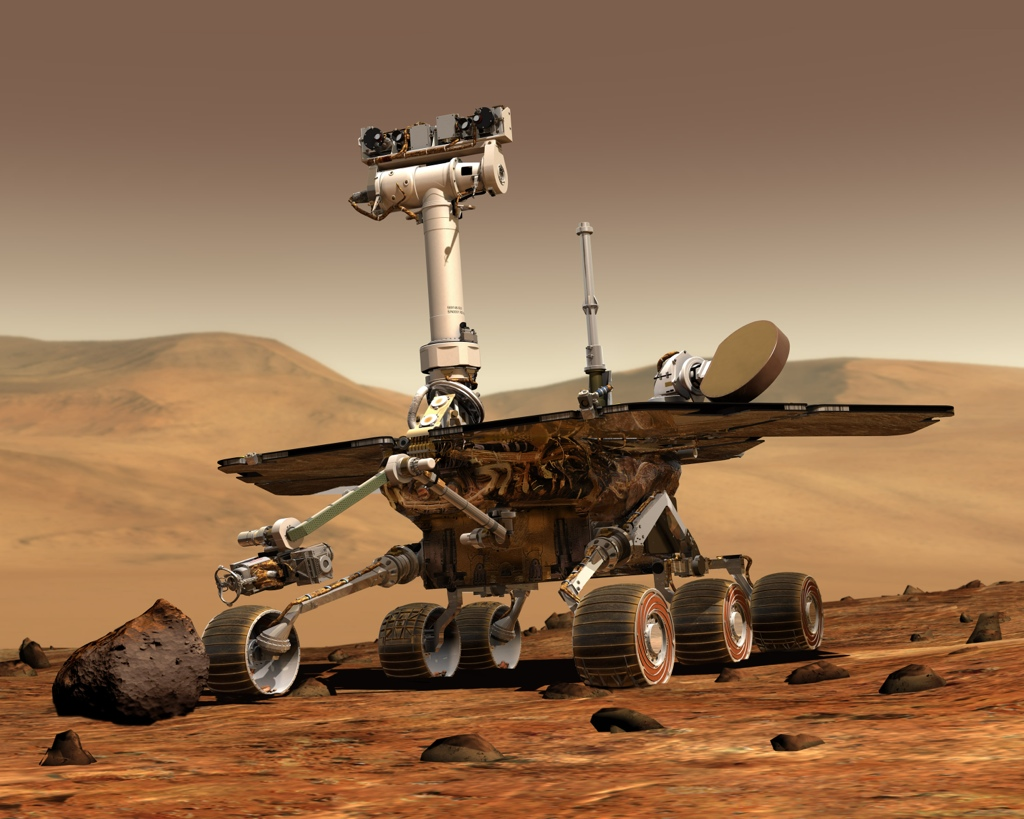
\includegraphics[width=6cm]{kapitel3/nasa_rover}
  \caption{Ein Nasa Rover}
  \label{Kap2:NasaRover}
\end{figure}


Man kann sich auch selber ein Makro für das Einfügen von Bildern schreiben:

\bild{kapitel3/modell_point_to_point}{6cm}{Point to Point}

\begin{sidewaysfigure}
 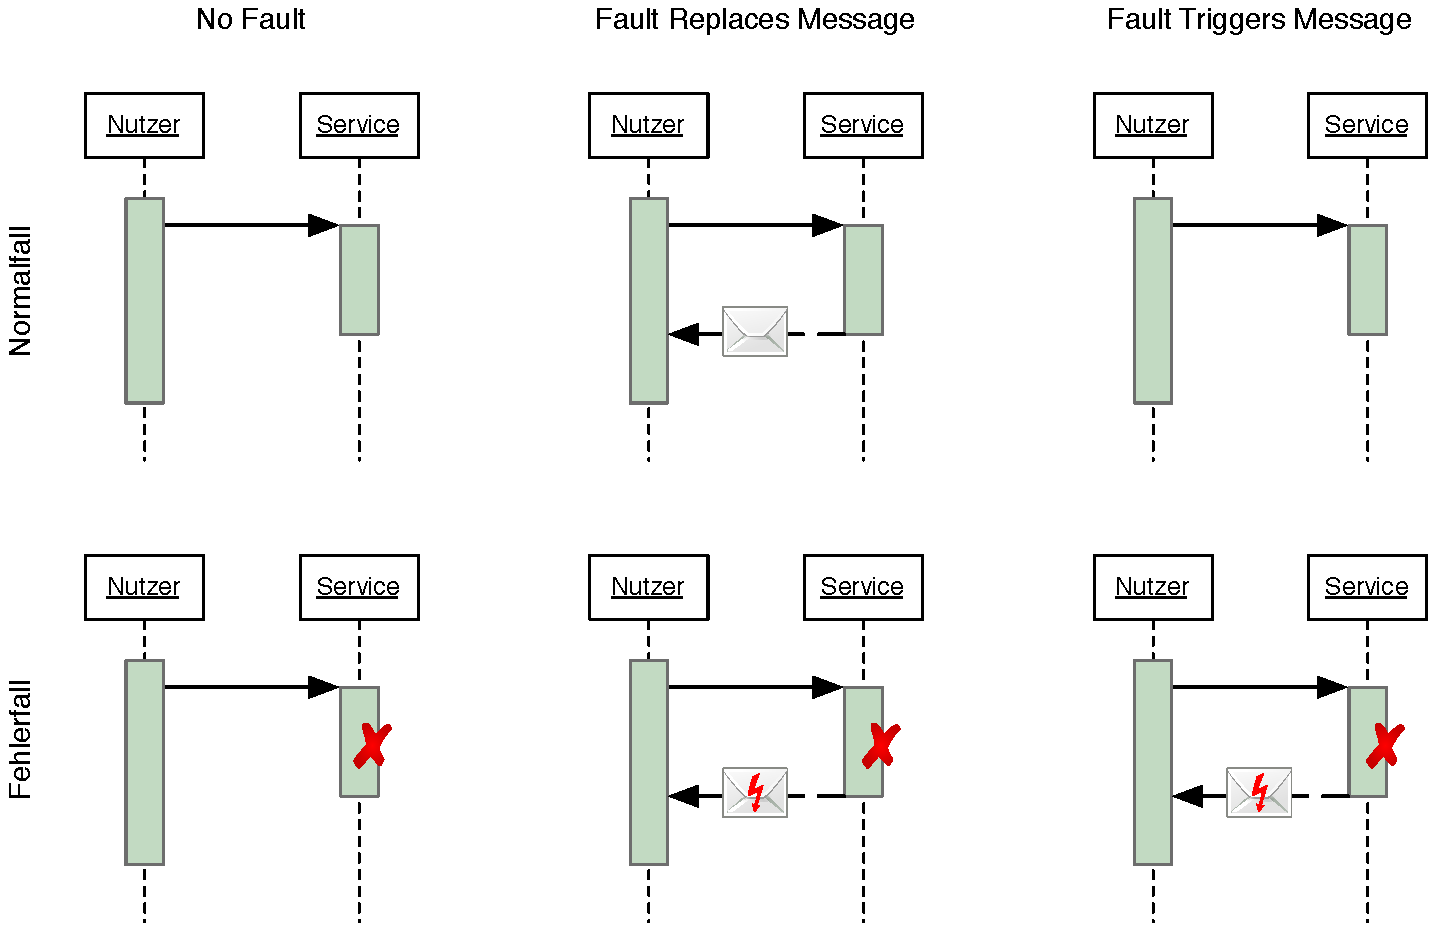
\includegraphics[width=22cm]{kapitel3/ws-wsdl20-fehler}
  \caption{Sehr große Grafiken kann man drehen, damit sie auf die Seite passen}
  \label{Kap2:wsdl-fehler}
\end{sidewaysfigure}


\clearpage % Alle Bilder, die bisher kamen ausgeben

\section{Formelsatz}

Eine Formel gefällig? Mitten im Text $a_2 = \sqrt{x^3}$ oder als eigener Absatz (siehe Formel~\ref{Formel}):

\begin{equation}
\begin{bmatrix}         
   1 &  4 &  2 \\
   4 &  0 & -3 
\end{bmatrix}        
        \cdot
\begin{bmatrix}                
   1 &  1 &  0 \\
  -2 &  3 &  5 \\
   0 &  1 &  4 
\end{bmatrix}        
       {=} 
\begin{bmatrix}               
  -7 &  15 &  28 \\
   4 &   1 & -12 
\end{bmatrix}
\label{Formel}
\end{equation}


\section{Sourcecode}

Man kann mit Latex auch ganz toll Sourcecode in den Text aufnehmen.

\subsection{Aus einer Datei}

\lstinputlisting[firstline=2,language=Java,caption={Crypter-Interface},label=lst:CrypterInterface]{\srcloc/Crypter.java}


\subsection{Inline}

\begin{lstlisting}[language=Java,caption=Methode checkKey()]
    /**
     * Testet den Schlüssel auf Korrektheit: Er muss mindestens die Länge 1
     * haben und darf nur Zeichen von A-Z enthalten.
     *
     * @param key zu testender Schlüssel
     * @throws CrypterException wenn der Schlüssel nicht OK ist.
     */
    protected void checkKey(Key key) throws CrypterException {

        // Passt die Länge?
        if (key.getKey().length == 0) {
            throw new CrypterException("Der Schlüssel muss mindestens " +
                    "ein Zeichen lang sein");
        }

        checkCharacters(key.getKey(), ALPHABET);
    }
\end{lstlisting}


\section{Anforderungen}

Anforderungen im Format des Volere-Templates (Snowcards) \autocite{Volere} können per Makro eingefügt werden.

\snowcard % Snowcard einbinden (Anpassungen in titelblatt.tex)
   {F52} % Nummer des Requirements
   {F} % Art
   {Hoch} % Priorität
   {User Authentifizierung} % Titel
   {Interview mit Abteilungsleiter} % Herkunft (Optional)
   {F12} % Konflikte (Optional)
   {Der Benutzer ist in der Lage sich über seinen
    Benutzernamen und sein Passwort am System anzumelden} % Beschreibung
   {Ein Benutzer kann sich mit seinem Firmenweiten Benutzernamen und
   Passwort über die Anmeldemaske anmelden und hat Zugriff auf die
   Funktionen des Systems} % Fit-Kriterium (Optional)
   {Benutzerhandbuch des Altsystems} % Material (Optional)

Ebenso nicht-funktionale Anforderungen mit Hilfe von Quality Attribute Scenarios. Siehe hierzu \autocite{Barbacci2003}.

\qas % Quality-Attribute Scenario einbinden (Anpassungen in titelblatt.tex)
   {NF11} % Nummer des Requirements
   {Hoch} % Priotität
   {Performance des Jahresabschlusses} % Titel
   {Endbenutzer} % Quelle
   {Startet einen Jahresabschluss} % Stimulus
   {Buchhaltungssystem} % Artefakt
   {Das System befindet sich im normalen Betriebszustand} % Umgebung
   {Jahresabschluss ist durchgeführt und kann als PDF abgerufen werden} % Antwort
   {10 Minuten} % Antwort-Maß

\newcommand{\highlightbox}[2]{%
    \colorbox{cyan!20}{%
        \parbox{#1}{\vspace{0.5em}\centering #2\vspace{0.5em}}%
    }%
}

\chapter{Suchproblem und Suchalgorithmen}

Ein Agent muss für ein bestimmtes Ziel die richtige Auswahl an Aktionen treffen und vorausschauend planen. Der Prozess der Bestimmung der Abfolge von Aktionen wird als Suche bezeichnet und mithilfe von Suchalgorithmen, wie A$^*$, durchgeführt. Für diesen Prozess benötigt der Agent einen Raum mit Regeln und Informationen, der im Suchproblem definiert wird. Die Informationen des folgenden Kapitel basieren auf den wissenschaftlichen Arbeiten \autocite{RN2020}, \autocite{4082128} und \autocite{Felner2011}.


\section{Suchproblem}

Ein Suchproblem wird durch einen Satz möglicher Zustände, einen Ausgangszustand, Zielzustände, Aktionen, ein Übergangsmodell und Aktionskosten definiert.

Die Zustände beschreiben die Umwelt des Agenten. Der Ausgangszustand $s$ gibt den Zustand an, von dem der Agent startet. Ein Agent verfolgt ein oder mehrere Ziele, die durch Zielzustände definiert werden.

\[
\highlightbox{0.9\textwidth}{$
    \begin{aligned}
			s = \{AtCover, GunLoaded, PlayerAlive\}
    \end{aligned}
$}
\]

Die Aktionen die ein Agent besitzt können in bestimmten Zuständen $ACTIONS(s)$ ausgeführt werden.

\[
\highlightbox{0.9\textwidth}{$
    \begin{aligned}
			ACTIONS(GunLoaded) &= \{Shoot\} \\
			ACTIONS(\lnot GunLoaded) &= \{Reload\}
    \end{aligned}
$}
\]

Ein Übergangsmodell $TRANSITION(s,a) = s^*$ beschreibt den resultierenden Zustand $s^*$ der durch Aktionen $a$ im derzeitigen Zustand $s$ resultiert.

\[
\highlightbox{0.9\textwidth}{$
    \begin{aligned}
			TRANSITIONS(GunLoaded, Shoot) &= \lnot PlayerAlive
    \end{aligned}
$}
\]

Durch eine Aktion-Kosten Funktion $ACTIONCOST(s,a,s^*)$ erhalten wir die Kosten einer Aktion $a$, welche in einem Zustand $s$ ausgeführt wird und in einen neuen Zustand $s^*$ resultieren.

Die Lösung für ein Suchproblem ist die Sequenz an Aktionen, also der Plan, der vom Ausgangszustand zum Zielzustand führen soll. Der gewählte Pfad sollte die geringsten Kosten unter allen möglichen Lösungen aufweisen und somit eine optimale Lösung darstellen. Der Satz an möglichen Zuständen kann dabei als Graph modelliert werden, wobei die Kanten die Aktionen und die Knoten die Zustände repräsentieren.


\section{Suchalgorithmen}

Das Suchproblem soll mit seinen Informationen durch einen Suchalgorithmus gelöst werden. Ein Suchalgorithmus erzeugt aus dem Suchproblem einen Suchbaum. Wie beim Graphen besteht ein Suchbaum aus Knoten $n$ und Kanten $a$, welche zu weiteren Knoten führen.


\subsection{Knoten eines Suchbaums}

Ein Knoten speichert dabei:
\begin{itemize}
	\item Einen Zustand, zu dem die Aktion des jeweiligen Knoten geführt hat
	\item Eine Aktion, die auf dem Eltern-Knoten ausgeführt wurde
	\item Einen Eltern-Knoten, auf dem die Aktion durchgeführt wurde und den jeweiligen Knoten generiert hat
	\item Die Pfad-Kosten, der die summierten Kosten vom Ausgangsknoten bis zum jeweiligen Knoten speichert
\end{itemize}
Der Wurzelknoten ist dabei der Ausgangszustand des Agenten. Der Suchbaum beschreibt dabei Pfade zu Knoten und Ziel-Knoten, wobei mehrere Pfade zum selben Zustand führen können, jedoch jeder Knoten im Suchbaum einen eindeutigen Pfad zurück zur Wurzel hat.


\subsection{Expansion eines Suchalgorithmus}

Bei der Expandierung betrachet der Suchalgorithmus über die Funktion $TRANSITIONS(n)$ alle möglichen Kanten $ACTIONS(n)$ des aktuellen Knotens $n$ an. Zu den Kanten werden die entsprechenden Kind-Knoten generiert und einer offene-Liste (\textit{open list}) hinzugefügt. Der Suchalgorithmus wählt den nächsten Knoten zur Expansion aus der offenen Liste aus, basierend auf dem jeweiligen Suchverfahren und dessen Bewertungsfunktion $f(n)$.

Im Bereich der Suchalgorithmen wird zwischen informierten und uniformierten Algorithmen unterschieden. Informierte Algorithmen können dabei die Distanz zum Ziel über eine Heuristik schätzen, während uniformierte eine solche Schätzung nicht durchführen können. Unter die uninformierten Suchalgorithmen fallen beispielsweise die Breitensuche, Dijkstra und Tiefensuche. Zu den informierten Suchalgorithmen gehören unter anderem \textit{Greedy best-first-search} und der A* Algorithmus. Informierte Suchalgorithmen können einen Pfad durch die Informationen der Heuristik effizienter finden, als uninformierte Suchalgorithmen.

\begin{figure}[h]
  \centering
  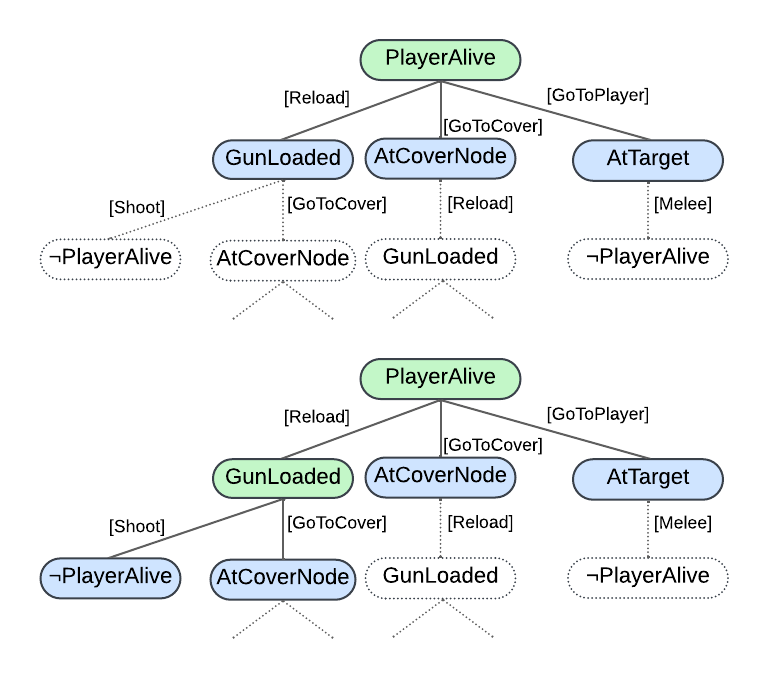
\includegraphics[width=15cm]{Suchalgorithmen/SAS}
	\captionsetup{justification=justified, format=plain}
  \caption{Suchbaum: Fängt vom Ausgangszustand an und soll den Zielzustand $\lnot \textit{PlayerAlive}$ erreichen. Grüne Knoten sind expandierte Knoten, welche in eine geschlossene Liste hinzugefügt werden. Blaue Knoten sind offene gefundene Nachbarknoten aus der offenen-Liste. Gestrichelte Knoten sind nicht entdeckte Knoten. Im Falle des Beispiels hat sich der Suchalgorithmus für den Knoten GunLoaded entschieden, da dieser optimaler als andere Nachbarknoten ist. Von dort aus ist der Zielzustand erreichbar und der Algorithmus würde eine Sequenz von Aktionen geben: \textit{[Reload,Shoot]}}
  \label{Suchalgorithmen}
\end{figure}
\clearpage

\subsection{A* Algorithmus}

Gehört zu den informierten und heuristischen Suchverfahren. Er ist ein so genannter vollständiger Algorithmus und findet einen Pfad zur Lösung, wenn einer vorhanden ist. Der Einsatz des Algorithmus wird oft für Routenplaner benutzt. So benutzt Godot 4.3 den A* Algorithmus für die Navigation von NPC. Der GOAP benutzt A*, um eine optimale Sequenz von Aktionen zu finden, welche das Ziel erfüllen.

\subsubsection{Bewertungsfunktion}

Suchalgorithmen, wie A* benutzen eine Bewertungsfunktion $f(n)$, welche dazu dient die Priorität eines Knoten $n$ während der Suche zu bewerten. Es werden dabei alle Pfad-Kosten $g(n)$ vom Ausgangsknoten bis zum Knoten $n$ mit der Heuristik $h(n)$ des Knoten $n$ summiert.

\[
\highlightbox{0.9\textwidth}{$
    \begin{aligned}
			f(n) = g(n) + h(n)
    \end{aligned}
$}
\]

Mit jeder Erweiterung des Pfades von $n$ zu $n^{\ast}$ steigen die Kosten $g(n)$. Dies liegt an den positiven tatsächlichen Aktion-Kosten $ACTIONCOST(n,a,n^*)$ der Kanten zwischen den Knoten .

\[
\highlightbox{0.9\textwidth}{$
    \begin{aligned}
			g(n) + ACTIONCOST(n,a,n^*) + h(n^*) &= g(n^*) + h(n^*)
    \end{aligned}
$}
\]

\subsubsection{Heuristik}

Ein Suchalgorithmus sollte einen Pfad mit möglichst geringen Kosten, den optimalen-Pfad, zum Ziel finden. Ob A* einen optimalen Pfad findet, hängt von den Eigenschaften der Heuristik $h(n)$ ab. Eine Heuristik weist die Eigenschaften der Zulässigkeit und Konsistenz auf.
Bei einer zulässigen Heuristik werden die Kosten stets unterschätzt oder genau geschätzt. Sie bleibt im Intervall $[0, h^{\ast}(n)]$ wobei $h^{\ast}(n)$ die tatsächlichen Kosten sind.

\[
\highlightbox{0.9\textwidth}{$
    \begin{aligned}
			0 \leq h(n) \leq h^*(n)
    \end{aligned}
$}
\]

Eine konsistente Heuristik, muss gleichzeitig zulässig sein und die Dreiecksungleichung erfüllen. Umgekehrt muss eine zulässige Heuristik nicht konsistent sein. So muss diese die Dreiecksungleichung erfüllen, welche besagt, dass die Heuristik $h(n)$ geringer sein soll als die Summe der Aktion $a$ und die Heuristik des folgenden Knoten $h(n^*)$.

\[
\highlightbox{0.9\textwidth}{$
    \begin{aligned}
			h(n) \leq ACTIONCOST(n,a,n^*) + h(n^*)
    \end{aligned}
$}
\]

Die konsistente Heuristik weist eine stärkere Eigenschaft auf als eine zulässige Heuristik. Der expandierte Knoten bei einer konsistenten Heuristik wird optimal sein, wodurch dieser Knoten nicht erneut in die offene-Liste hinzufügt werden muss.

Mit einer inkonsistenten Heuristik können Pfade auftreten, welche denselben Zustand erreichen. Somit können mehrere Pfade mit unterschiedlichen Kosten, aber demselben Zustand in der offenen Liste auftreten, was zur höheren Zeit. und Speicherkosten führt.

\subsubsection{Beweis für Optimalität}

Arbeitet der A* Algorithmus mit einer zulässigen oder konsistenten Heuristik, so wird diese den optimalen, kostengünstigsten Pfad zu einem Ziel finden.

Vorraussetzung:
\begin{itemize}
\item A* expandiert auf Knoten mit der geringsten $f(n)$
\item Wir haben zwei mögliche Zielknoten:
\begin{itemize}
	\item optimaler Zielknoten: $G_o$
	\item suboptimaler Zielknoten: $G_s_o$
\end{itemize}
\item Eine zulässige Heuristik: $0 \leq h(n) \leq h^*(n)$
\item Einen nicht expandierten Knoten: $n$
\end{itemize}

Beweis:
\begin{enumerate}
	\item Da keine weiteren Schritte vom Zielzustand möglich sind gilt: $h(G_o) \land h(G_s_o) = 0$
	\[
	\highlightbox{0.9\textwidth}{$
		\begin{align*}
			f(G_o) &= g(G_o) + h(G_o) \\
			f(G_o) &= g(G_o) \\
			f(G_s_o) &= g(G_s_o) + h(G_s_o) \\
			f(G_s_o) &= g(G_s_o)
		\end{align*}
	$}
	\]
	
	Da $G_s_$ suboptimal ist folgt, dass die Pfadkosten $f(n)$ von $G_s_o > G_o$ sind und somit: $f(G_s_o) > f(G_o)$.
	\item Da $g(G_o)$ der tatsächliche Zielknoten ist und $h^*(n)$ die tatsächlichen Kosten von $G_o$ sind gilt:
	\[
	\highlightbox{0.9\textwidth}{$
    \begin{align*}
			f(n) = g(n) + h(n) &< g(n) + h^*(n) = g(G_o) \\
			f(n) &< g(G_o)
		\end{align*}
	$}
	\]
\end{enumerate}
Aus 1. und 2. folgt: $f(n) < f(G_o) < f(G_s_o)$. Somit würde A* nicht zu $G_s_o$ führen und ist mit einer zulässigen Heuristik optimal.

\begin{figure}[h]
  \centering
  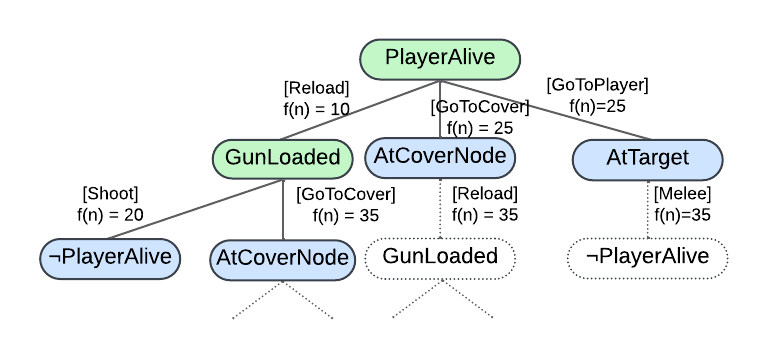
\includegraphics[width=15cm]{Suchalgorithmen/A_Erweiterung}
	\captionsetup{justification=justified, format=plain}
  \caption{A Suchalgorithmus: Der Pfad \textit{[Reload,Shoot]} hat mit $f(n)=20$ die geringsten Pfadkosten. Das Beispiel kommt aus  Abbildung 1.1. Wie genau $g(n)$ und $h(n)$ am Beispiel von NPC-Aktionen berechnet wird, wird im GOAP Kapitel erklärt.}
  \label{Suchalgorithmen}
\end{figure}
%\usepackage{pgfplots}
\usepackage{csvsimple}

\pgfplotsset{compat=1.17}

\chapter{Grafik}

\begin{tikzpicture}
    \begin{axis}[
        width=15cm,
        height=15cm,
        xlabel={NPC-Anzahl},
        ylabel={Durchschnittliche FPS},
        title={Durchschnittliche FPS der Entscheidungssysteme},
        grid=major,
        legend style={at={(1.05,1)}, anchor=north west, font=\footnotesize}, % Anpassen der Schriftgröße der Legende
        enlarge x limits=0.1, % Etwas mehr Platz für die x-Achse
        enlarge y limits=0.1  % Etwas mehr Platz für die y-Achse
    ]
    \addplot 
        table [x=NPC, y=FPS, col sep=comma] {csv/goap\_plot\_data.csv};
    \addlegendentry{GOAP}
    
    \addplot 
        table [x=NPC, y=FPS, col sep=comma] {csv/fsm\_plot\_data.csv};
    \addlegendentry{FSM}
    
    \addplot 
        table [x=NPC, y=FPS, col sep=comma] {csv/bt\_plot\_data.csv};
    \addlegendentry{BT}
    \end{axis}
\end{tikzpicture}
%\chapter{Schreibstil}

\section{Fremdsprachige Begriffe}

Wenn Sie Ihre Arbeit auf Deutsch verfassen, gehen Sie sparsam mit englischen Ausdrücken um. Natürlich brauchen Sie etablierte englische Fachbegriffe, wie z.\,B. \textit{Interrupt}, nicht zu übersetzen. Sie sollten aber immer dann, wenn es einen gleichwertigen deutschen Begriff gibt, diesem den Vorrang geben. Den englischen Begriff (\textit{term}) können Sie dann in Klammern oder in einer Fußnote\footnote{Englisch: \textit{footnote}.} erwähnen. Absolut unakzeptabel sind deutsch gebeugte englische Wörter oder Kompositionen aus deutschen und englischen Wörtern wie z.\,B. downgeloadet, upgedated, Keydruck oder Beautyzentrum.


\section{Zitate}

\subsection{Zitate im Text}

Wichtig ist das korrekte Zitieren von Quellen, wie es auch von \cite{Kornmeier2011} dargelegt wird. Interessant ist in diesem Zusammenhang auch der Artikel von \cite{Kramer2009}. Häufig werden die Zitate auch in Klammern gesetzt, wie bei \parencite{Kornmeier2011} und mit Seitenzahlen versehen \parencite[S. 22--24]{Kornmeier2011}.

Bei Webseiten wird auch die URL und das Abrufdatum mit angegeben \parencite{Gao2017}. Wenn die URL nicht korrekt umgebrochen wird, lohnt es sich, an den Parametern \textit{biburl*penalty} in der \texttt{preambel.tex} zu drehen. Kleinere Werte erhöhen die Wahrscheinlichkeit, dass getrennt wird.

\subsection{Zitierstile}

Verwenden Sie eine einheitliche und im gesamten Dokument konsequent durchgehaltene Zitierweise\index{Zitierweise}. Es gibt eine ganze Reihe von unterschiedlichen Standards für das Zitieren und den Aufbau eines Literaturverzeichnisses. Sie können entweder mit Fußnoten oder Kurzbelegen im Text arbeiten. Welches Verfahren Sie einsetzen ist Ihnen überlassen, nur müssen Sie es konsequent durchhalten.

In der Informatik ist das Zitieren mit Kurzbelegen\index{Zitat!Kurzbeleg} im Text (Harvard"=Zitierweise) weit verbreitet, wobei für das Literaturverzeichnis häufig die Regeln der \acs{ACM} oder \acs{IEEE} angewandt werden.\footnote{Einen Überblick über viele verschiedene Zitierweisen finden Sie in der \url{http://amath.colorado.edu/documentation/LaTeX/reference/faq/bibstyles.pdf}}

Am einfachsten ist es, wenn Sie das \verb+\autocite{}+-Kommando verwenden. Bei diesem Kommando können Sie in der Datei \texttt{perambel.tex} festlegen, wie die Zitate generell aussehen sollen, \zb \ ob sie in Fußnoten erfolgen sollen oder nicht. Wollen Sie von dem globalen Zitierstil abweichen, können Sie weiterhin spezielle Kommandos benutzen:

\begin{itemize}
	\item \verb+\autocite{Willberg1999}+: \autocite{Willberg1999}
	\item \verb+\cite{Willberg1999}+: \cite{Willberg1999}
	\item \verb+\parencite{Willberg1999}+: \parencite{Willberg1999}
	\item \verb+\footcite{Willberg1999}+: \footcite{Willberg1999}
	\item \verb+\citeauthor{Willberg1999}+: \citeauthor{Willberg1999}
	\item \verb+\citeauthor*{Willberg1999}+: \citeauthor*{Willberg1999}
	\item \verb+\citetitle{Willberg1999}+: \citetitle{Willberg1999}
	\item \verb+\fullcite{Willberg1999}+: \fullcite{Willberg1999}
\end{itemize}

Denken Sie daran, dass das Übernehmen einer fremden Textstelle ohne entsprechenden Hinweis auf die Herkunft in wissenschaftlichen Arbeiten nicht akzeptabel ist und dazu führen kann, dass die Arbeit nicht anerkannt wird. Plagiate\index{Plagiat!Bewertung} werden mit mangelhaft (5,0) bewertet und können weitere rechtliche Schritte nach sich ziehen.


\subsection{Zitieren von Internetquellen}

Internetquellen\index{Zitat!Internetquellen} sind normalerweise \textit{nicht} zitierfähig. Zum einen, weil sie nicht dauerhaft zur Verfügung stehen und damit für den Leser möglicherweise nicht beschaffbar sind und zum anderen, weil häufig der wissenschaftliche Anspruch fehlt.\footnote{Eine lesenswerte Abhandlung zu diesem Thema findet sich (im Internet) bei \cite{Weber2006}}

Wenn ausnahmsweise doch eine Internetquelle zitiert werden muss, z.\,B. weil für eine Arbeit dort Informationen zu einem beschriebenen Unternehmen abgerufen wurden, sind folgende Punkte zu beachten:

\begin{itemize}
\item Die Webseite ist auszudrucken und im Anhang der Arbeit beizufügen,
\item das Datum des Abrufs und die URL sind anzugeben,
\item verwenden Sie Internet"=Seiten ausschließlich zu illustrativen Zwecken (z.\,B. um einen Sachverhalt noch etwas genauer zu erläutern), aber nicht zur Faktenvermittlung (z.\,B. um eine Ihrer Thesen zu belegen).
\end{itemize}

Wenn Sie aufgrund der Natur Ihrer Arbeit sehr viele Internetquellen benötigen, dann können Sie diese statt sie auszudrucken auch in elektronischer Form abgeben (CD/DVD). Als Abgabeformat der elektronischen Quellen ist PDF/A\footnote{Bei PDF/A handelt es sich um ein besonders stabile Variante des \ac{PDF}, die von der  \ac{ISO} standardisiert wurde.} vorteilhaft, weil es von allen Formaten die größte Stabilität besitzt.
Auf der CD/DVD geben Sie bitte auch eine HTML"=Version des Literaturverzeichnisses ab, in der die Online"=Quellen sowie die gespeicherten PDF"=Dateien verlinkt sind.

Wikipedia\index{Zitat!Wikipedia} stellt einen immensen Wissensfundus dar und enthält zu vielen Themen hervorragende Artikel. Sie müssen sich aber darüber im Klaren sein, dass die Artikel in Wikipedia einem ständigen Wandel unterworfen sind und nicht als Quelle für wissenschaftliche Fakten genutzt werden sollten. Es gelten die allgemeinen Regeln für das Zitieren von Internetquellen. Sollten Sie doch Wikipedia nutzen müssen, verwenden Sie bitte ausschließlich den Perma"=Link\footnote{Sie erhalten den Permalink über die Historie der Seite und einen Klick auf das Datum.}\index{Permalink} zu der Version der Seite, die Sie aufgerufen haben.


% Jedes Kapitel besteht aus Unterkapiteln (section)
\section{Gliederung: Zweite Ebene}

Die Gliederung im Inhaltsverzeichnis erfolgt mit Kapiteln \verb+\chapter{Titel}+, Abschnitten \verb+\section{Titel}+, Unterabschnitten \verb+\subsection{Titel}+. Zusätzlich können noch Unterunterabschnitte \verb+\subsubsection{Titel}+ und Absätze \verb+\paragraph{Titel}+ verwendet werden. Damit kommt man auf maximal fünf Ebenen, was für eine Abschlussarbeit mehr als ausreichend ist.

Auf jeder Ebene sollten Sie erläutern, was in den darunter liegenden Ebene beschrieben wird, sodass im Normalfall keine Gliederungsebene leer ist und nur aus Untereinheiten besteht. Im folgenden zeigt dieses Template, wie man weitere Ebenen mit \LaTeX erzeugt.

% Unterkapitel können noch einmal durch subsections untergliedert
% werden (jetzt auf der 3. Ebene)
\subsection{Gliederung: Dritte Ebene}

% Mit Labels können Sie sich später im Text wieder auf diese Stelle beziehen
\label{Gliederung:EbeneDrei}

% Einträge für den Index anlegen. Ein Index wird normalerweise in einer Abschluss-
% arbeit nicht benötigt.
\index{Gliederung!Ebenen}

% Auf der 4. Ebene liegen die subsubsections. In diesem Template bekommt die
% 4. Ebene keinen Nummern mehr und erscheint auch nicht im Inhaltsverzeichnis.
\subsubsection{Gliederung: Vierte Ebene}

% Auf der 5. Ebene werden einzelne Absätze mit Überschriften versehen.
\paragraph{Gliederung: Fünfte Ebene} Anders als in diesem Beispiel, darf in Ihrer Arbeit kein Gliederungspunkt auf seiner Ebene alleine stehen. D.\,h. wenn es ein 1.1 gibt, muss es auch ein 1.2 geben.
 % Externe Datei einbinden
%\chapter{Typografie}

\section{Hervorhebungen}
\label{Einleitung:Textauszeichnungen}

Achten Sie bitte auf die grundlegenden Regeln der Typografie\index{Typografie}\footnote{Ein Ratgeber in allen Detailfragen ist \cite{Forssman2002}.}, wenn Sie Ihren Text schreiben. Hierzu gehören z.\,B. die Verwendung der richtigen "`Anführungszeichen"' und der Unterschied zwischen Binde- (-), Gedankenstrich (--) und langem Strich (---). Sie erhalten den Bindestrich in \LaTeX{} mit \verb+-+, den Gedankenstrich mit \verb+--+ und den langen Strich mit \verb+---+.

Wenn Sie Text hervorheben wollen, dann setzten Sie ihn mit \verb+\textit+ \textit{kursiv} (Italic) und nicht \textbf{fett} (Bold). Fettdruck ist Überschriften vorbehalten; im Fließtext stört er den Lesefluss. Das \underline{Unterstreichen} von Fließtext ist im gesamten Dokument tabu und kann maximal bei Pseudo"=Code vorkommen.\index{Hervorhebungen}


\section{Anführungszeichen}

Deutsche Anführungszeichen werden mit \verb+"`+ und \verb+"'+ erzeugt: "`dieser Text steht in \glq Anführungszeichen\grq; alles klar?"'. Englische Anführungszeichen hingegen mit \verb+``+ und \verb+''+: ``this is an `English' quotation''. Beachten Sie, dass Sie in Zitaten immer die zur Sprache passenden Anführungszeichen verwenden. Die Verwendung von \verb+"+ ist für Anführungszeichen immer falsch und führt bei \LaTeX{} zu seltsamen "Effekten".

Um sich diesen Ärger zu sparen, biete sich die Verwendung des Paketes \textit{csquotes} und des Kommandos \verb+\enquote+ an. Hierdurch werden die Anführungszeichen korrekt für die eingestellte Sprache gesetzt und Sie müssen sich \enquote{keine Sorgen mehr über die \enquote{Anführungszeichen} machen}.


\section{Silbentrennung}
\index{Silbentrennung}
\LaTeX{} führt eine automatische Silbentrennung durch, sodass Sie sich eigentlich um nichts kümmern müssen. Allerdings werden Wörter, die bereits einen Bindestrich enthalten nicht getrennt, z.\,B. Datenschutz-Grundverordnung. Wenn Sie Ihren Text auf Deutsch schreiben, können Sie dann alternativ \verb+"=+ für den Bindestrich im Wort verwenden, z.\,B. \\
\verb+Datenschutz"=Grundverordnung+, damit \LaTeX{}  weiterhin richtig trennt.

Ist die Silbentrennung aus einem anderen Grund nicht erfolgt, z.\,B. weil das Wort nur aus Großbuchstaben besteht, sodass die Zeile über den rechten Rand hinaussteht (Sie bekommen eine \textit{overfull hbox}-Warnung), können Sie \LaTeX{} helfen, indem Sie weitere Trennstellen angeben. Dies geschieht durch \verb+"-+ als Zeichen, z.\,B. \verb+Staats"-ver"-trag+.

\section{Abkürzungen}
\index{Abkürzungen}
\index{Abbreviation|see{Abkürzungen}}

Eine \gls{abk} (\verb+\gls{abk}+) wird bei der ersten Verwendung ausgeschrieben. Danach nicht mehr: \gls{abk}. Man kann allerdings mit \verb+\acrlong{abk}+ die Langform explizit anfordern (\acrlong{abk}) oder mit \verb+\acrshort{abk}+ die Kurzform (\acrshort{abk}) oder mit \verb+\acrfull{abk}+ auch noch einmal die Definition (\acrfull{abk}). Wenn Sie eine Abkürzung im Plural verwenden wollen, gibt ihnen \verb+\glspl{isp}+ die Möglichkeit (\glspl{isp}).

Das Abkürzungsverzeichnis muss aufgrund der automatischen Sortierung separat kompiliert werden. Der dazugehörige Befehl lautet:
\begin{verbatim}
makeindex -s %.ist -t %.alg -o %.acr %.acn
\end{verbatim}

Beachten Sie, dass bei Abkürzungen, die für zwei Wörter stehen, ein schmales Leerzeichen nach dem Punkt kommt (\verb+\,+ in \LaTeX{}): z.\,B. bzw. \zb{} und d.\,h. bzw. \dahe{}. Das Template bietet hierfür die beiden Makros \verb+\zb{}+ und \verb+\dahe{}+.


\section{Glossar}
Ein Eintrag in dem Glossar kann mithilfe des Befehls \verb*|\gls{glos:amplification}| erzeugt werden. Hierbei wird die Begriffserklärung in der Datei \texttt{/kapitel/glossar} verwendet und in dem Verzeichnis aufgeführt. Ein Beispiel hierfür wäre: \gls{glos:amplification}. Das Wort Amplification erscheint nun in der Begriffserklärung.

Das Glossar muss aufgrund der automatischen Sortierung separat kompiliert werden. Der dazugehörige Befehl lautet:
\begin{verbatim}
	"makeindex.exe" -s %.ist -t %.glg -o %.gls %.glo
\end{verbatim}



\section{Symbolverzeichnis}
Ein Eintrag in dem Symbolverzeichnis kann mithilfe des Befehls \verb*|\gls{symb:Pi}| erzeugt werden. Hierbei wird das Symbol in der Datei \texttt{/kapitel/symbole} geladen und in dem Verzeichnis aufgeführt. Ein Beispiel hierfür ist: \gls{symb:Pi} und \gls{symb:energyconsump}.

Das Symbolverzeichnis muss aufgrund der automatischen Sortierung separat kompiliert werden. Der dazugehörige Befehl lautet:

\begin{verbatim}
	"makeindex.exe" -s %.ist -t %.slg -o %.syi %.syg
\end{verbatim}


\section{Querverweise}

Querverweise auf eine Kapitelnummer macht man im Text mit \verb+\ref+ (Kapitel~\ref{Einleitung:Textauszeichnungen}) und auf eine bestimmte Seite mit \verb+\pageref+ (Seite~\pageref{Einleitung:Textauszeichnungen}). Man kann auch den Befehl \verb+\autoref+ benutzen, der automatisch die Art des referenzierten Elements bestimmt (\zb{} \autoref{Einleitung:Textauszeichnungen} oder \autoref{Kap2:Kopplungsformen}).


\section{Fußnoten}

Fußnoten werden einfach mit in den Text geschrieben, und zwar genau an die Stelle\footnote{An der die Fußnote auftauchen soll}. Hierzu dient der Befehl \verb+\footnote{Text}+.


\section{Tabellen}

Tabellen werden normalerweise ohne vertikale Striche gesetzt, sondern die Spalten werden durch einen entsprechenden Abstand voneinander getrennt.\footnote{Siehe \cite[S. 89]{Willberg2021}.} Zum Einsatz kommen ausschließlich horizontale Linien (siehe \autoref{Kap2:Kopplungsformen}).

\begin{table}[ht]
  \caption{Ebenen der Kopplung und Beispiele für enge und lose Kopplung}
  \label{Kap2:Kopplungsformen}
  \renewcommand{\arraystretch}{1.2}
  \small
  \centering
  \resizebox{\linewidth}{!}{ 
    \begin{tabular}{l l l}
    \toprule
    \textbf{Form der Kopplung} & \textbf{enge Kopplung} & \textbf{lose Kopplung}\\
    \midrule
    Physikalische Verbindung	&	Punkt-zu-Punkt	& 	über Vermittler\\
    Kommunikationsstil	&	synchron		&	asynchron\\
    Datenmodell	&	komplexe gemeinsame Typen	&	nur einfache gemeinsame Typen\\
    Bindung	&	statisch		&	dynamisch\\
    \bottomrule
    \end{tabular}
	}
\end{table}

Eine Tabelle fließt genauso, wie auch Bilder durch den Text. Siehe \autoref{Kap2:Kopplungsformen}.

Manchmal möchte man Tabellen, in denen der Text in der Tabellenspalte umbricht. Hierzu dient die Umgebung \texttt{tabularx}, wobei \texttt{L} eine Spalte mit Flattersatz und \texttt{X} eine mit Blocksatz definiert. Die Breite der Tabelle kann über den Faktor vor \verb+\textwidth+ angegeben werden.

\begin{table}[ht]
  \caption{Teildisziplinen der Informatik}
  \label{Kap2:Teildisziplinen}
  \renewcommand{\arraystretch}{1.2}
  \centering
  \small
    \begin{tabularx}{0.95\textwidth}{l X L}
      \toprule
      \textbf{Gebiet} & \textbf{Definition} & \textbf{Beispiel}\\
      \toprule
      \emph{Praktische Informatik} & Informatik-Disziplinen, welche sich vorwiegend mit der Entwicklung und Anwendung der Software-Komponenten befassen & Programmentwicklung, Compilerbau; im Aufbau von z.B. Informationssystemen und Netzwerken ergeben sich Überlappungen mit der technischen Informatik \\\midrule
      \emph{Technische Informatik} & Informatik-Disziplinen, welche sich vorwiegend mit der Entwicklung und Anwendung der Hardware-Komponenten befassen & Digitaltechnik, Mikroprozessortechnik \\\midrule
      \emph{Theoretische Informatik} & Informatik-Disziplinen, welche sich mit der Entwicklung von Theorien und Modellen der Informatik befassen und dabei viel Substanz aus der Mathematik konsumieren & Relationenmodell, Objekt-Paradigmen, Komplexitätstheorie, Kalküle \\\midrule
      \emph{Angewandte Informatik} & Informatik als instrumentale Wissenschaft & Rechtsinformatik, Wirtschaftsinformatik, Geoinformatik \\
      \bottomrule
    \end{tabularx}
\end{table}

Manchmal kommt es vor, dass eine Tabelle so lang wird, dass sie sich über mehr als eine Seite erstreckt. In diesem Fall können Sie das Paket \texttt{longtable} verwenden und die Tabelle mit \verb+\begin{longtable}[h]+ definieren. Die Tabelle wird dann \textit{nicht} in eine \texttt{table}-Umgebung eingeschlossen. Siehe hierzu \autoref{laendercodes} in \autoref{AnhangA}.


\section{Harveyballs}

\begin{quote}
    Harvey Balls sind kreisförmige Ideogramme, die dazu dienen, qualitative Daten anschaulich zu machen. Sie werden in Vergleichstabellen verwendet, um anzuzeigen, inwieweit ein Untersuchungsobjekt sich mit definierten Vergleichskriterien deckt. \parencite{Wikipedia_HarveyBalls}
\end{quote}

\begin{table}[ht]
  \caption{Beispiel für Harvey Balls}
  \label{tab:harveyexample}
  \centering
  \begin{tabular}{lccc}
    \toprule
    & Ansatz 1 & Ansatz 2 & Ansatz 3\\
    \midrule
    Eigenschaft 1	& \harveyBallNone & \harveyBallQuarter & \harveyBallHalf \\
    Eigenschaft 2	& \harveyBallHalf & \harveyBallThreeQuarter & \harveyBallFull \\
    Eigenschaft 3	& \harveyBallFull & \harveyBallThreeQuarter & \harveyBallQuarter\\
    \bottomrule
  \end{tabular}
\end{table}


\section{Aufzählungen}

Aufzählungen sind toll.

\begin{itemize}
  \item Ein wichtiger Punkt
  \item Noch ein wichtiger Punkt
  \item Ein Punkt mit Unterpunkten
    \begin{itemize}
      \item Unterpunkt 1
      \item Unterpunkt 2
    \end{itemize}
  \item Ein abschließender Punkt ohne Unterpunkte
\end{itemize}


Aufzählungen mit laufenden Nummern sind auch toll.

\begin{enumerate}
  \item Ein wichtiger Punkt
  \item Noch ein wichtiger Punkt
  \item Ein Punkt mit Unterpunkten
    \begin{enumerate}
      \item Unterpunkt 1
      \item Unterpunkt 2
    \end{enumerate}
  \item Ein abschließender Punkt ohne Unterpunkte
\end{enumerate}


Aufzählungen mit eigenen Bezeichnern sind auch toll.
\begin{enumerate}[label=RQ~\arabic*), leftmargin=1.75cm]
	\item Ein wichtiger Punkt
	\item Noch ein wichtiger Punkt
	\item Ein Punkt mit Unterpunkten
	\item Ein abschließender Punkt ohne Unterpunkte
\end{enumerate}


Auch die Auflistung im Fließtext ist sehr wertvoll: \begin{enumerate*}[label=\alph *)] \item wichtiger Punkt, \item zweiter wichtiger Punkt und \item der letzte Punkt. \end{enumerate*}


 % Externe Datei einbinden
%\chapter{Einbinden von Grafiken und Sourcecode}
\label{Kap3}

\section{Bilder}

Natürlich können auch Grafiken und Bilder eingebunden werden, siehe z.\,B. Abbildung~\ref{Kap2:NasaRover}.

\begin{figure}[h]
  \centering
  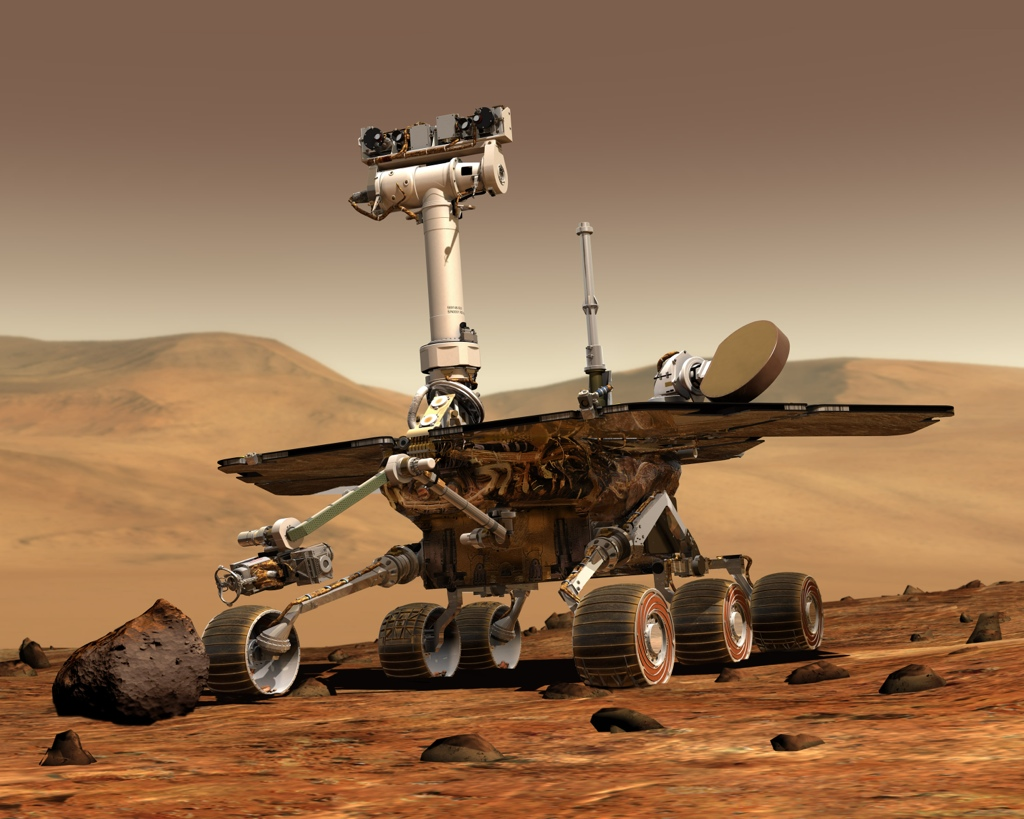
\includegraphics[width=6cm]{kapitel3/nasa_rover}
  \caption{Ein Nasa Rover}
  \label{Kap2:NasaRover}
\end{figure}


Man kann sich auch selber ein Makro für das Einfügen von Bildern schreiben:

\bild{kapitel3/modell_point_to_point}{6cm}{Point to Point}

\begin{sidewaysfigure}
 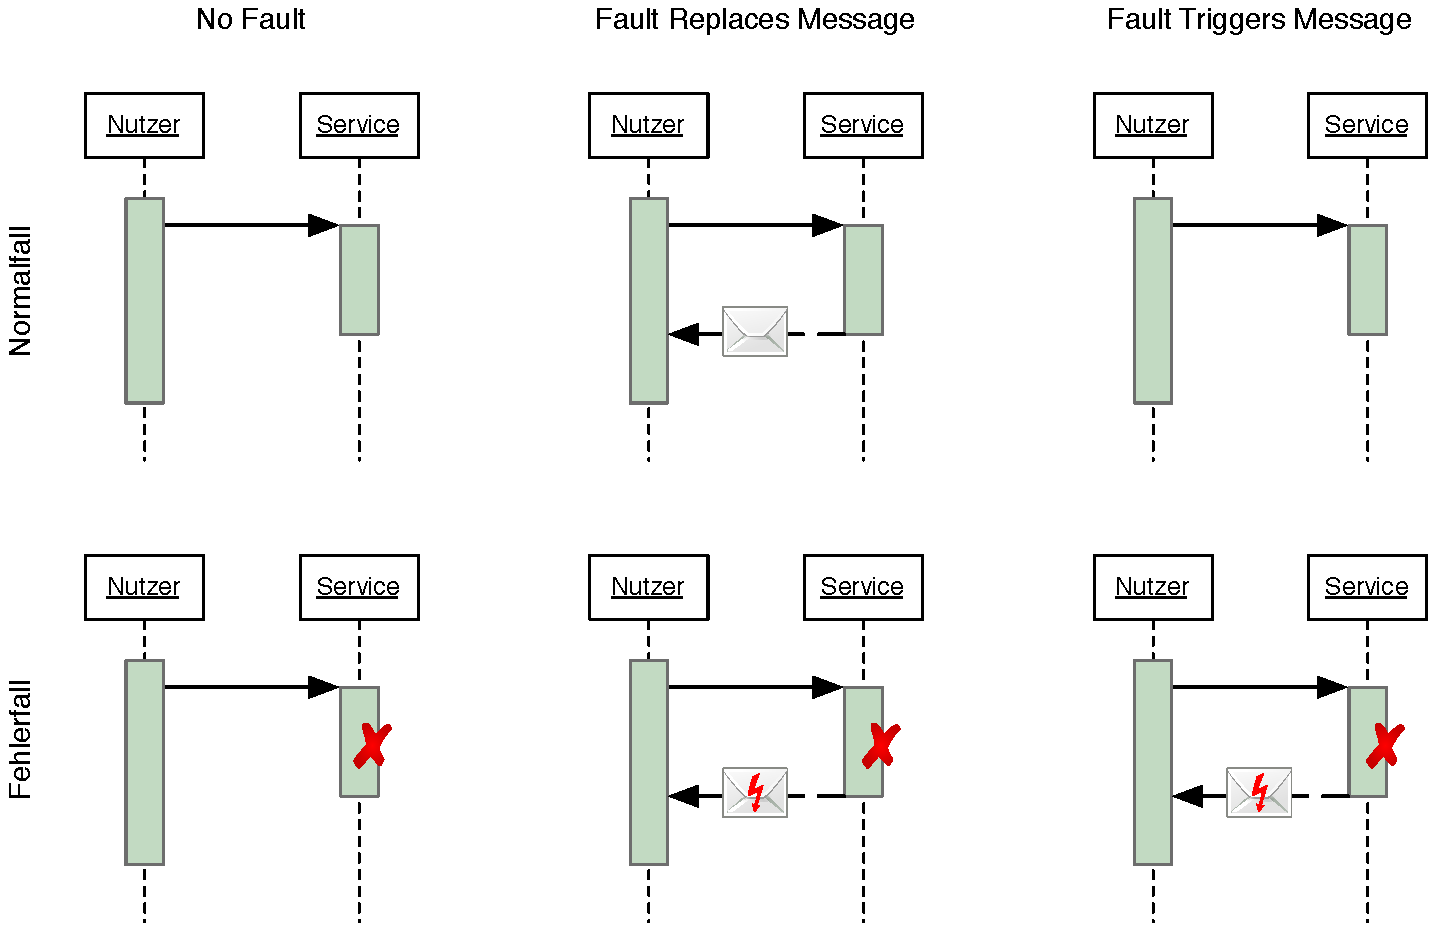
\includegraphics[width=22cm]{kapitel3/ws-wsdl20-fehler}
  \caption{Sehr große Grafiken kann man drehen, damit sie auf die Seite passen}
  \label{Kap2:wsdl-fehler}
\end{sidewaysfigure}


\clearpage % Alle Bilder, die bisher kamen ausgeben

\section{Formelsatz}

Eine Formel gefällig? Mitten im Text $a_2 = \sqrt{x^3}$ oder als eigener Absatz (siehe Formel~\ref{Formel}):

\begin{equation}
\begin{bmatrix}         
   1 &  4 &  2 \\
   4 &  0 & -3 
\end{bmatrix}        
        \cdot
\begin{bmatrix}                
   1 &  1 &  0 \\
  -2 &  3 &  5 \\
   0 &  1 &  4 
\end{bmatrix}        
       {=} 
\begin{bmatrix}               
  -7 &  15 &  28 \\
   4 &   1 & -12 
\end{bmatrix}
\label{Formel}
\end{equation}


\section{Sourcecode}

Man kann mit Latex auch ganz toll Sourcecode in den Text aufnehmen.

\subsection{Aus einer Datei}

\lstinputlisting[firstline=2,language=Java,caption={Crypter-Interface},label=lst:CrypterInterface]{\srcloc/Crypter.java}


\subsection{Inline}

\begin{lstlisting}[language=Java,caption=Methode checkKey()]
    /**
     * Testet den Schlüssel auf Korrektheit: Er muss mindestens die Länge 1
     * haben und darf nur Zeichen von A-Z enthalten.
     *
     * @param key zu testender Schlüssel
     * @throws CrypterException wenn der Schlüssel nicht OK ist.
     */
    protected void checkKey(Key key) throws CrypterException {

        // Passt die Länge?
        if (key.getKey().length == 0) {
            throw new CrypterException("Der Schlüssel muss mindestens " +
                    "ein Zeichen lang sein");
        }

        checkCharacters(key.getKey(), ALPHABET);
    }
\end{lstlisting}


\section{Anforderungen}

Anforderungen im Format des Volere-Templates (Snowcards) \autocite{Volere} können per Makro eingefügt werden.

\snowcard % Snowcard einbinden (Anpassungen in titelblatt.tex)
   {F52} % Nummer des Requirements
   {F} % Art
   {Hoch} % Priorität
   {User Authentifizierung} % Titel
   {Interview mit Abteilungsleiter} % Herkunft (Optional)
   {F12} % Konflikte (Optional)
   {Der Benutzer ist in der Lage sich über seinen
    Benutzernamen und sein Passwort am System anzumelden} % Beschreibung
   {Ein Benutzer kann sich mit seinem Firmenweiten Benutzernamen und
   Passwort über die Anmeldemaske anmelden und hat Zugriff auf die
   Funktionen des Systems} % Fit-Kriterium (Optional)
   {Benutzerhandbuch des Altsystems} % Material (Optional)

Ebenso nicht-funktionale Anforderungen mit Hilfe von Quality Attribute Scenarios. Siehe hierzu \autocite{Barbacci2003}.

\qas % Quality-Attribute Scenario einbinden (Anpassungen in titelblatt.tex)
   {NF11} % Nummer des Requirements
   {Hoch} % Priotität
   {Performance des Jahresabschlusses} % Titel
   {Endbenutzer} % Quelle
   {Startet einen Jahresabschluss} % Stimulus
   {Buchhaltungssystem} % Artefakt
   {Das System befindet sich im normalen Betriebszustand} % Umgebung
   {Jahresabschluss ist durchgeführt und kann als PDF abgerufen werden} % Antwort
   {10 Minuten} % Antwort-Maß
 % Externe Datei einbinden
%\chapter{Checkliste}
\label{Kap4}

Die folgende Checkliste kann dazu dienen, die Arbeit auf die wichtigsten Bewertungskriterien zu prüfen. Jeder Dozent hat andere Kriterien, die unten aufgeführten dürften aber für die meisten Dozenten gültig sein.

\section{Form und Sprache}

\begin{checklist}
  \footnotesize
  \item \textbf{Aufbau}: Die Arbeit ist nach wissenschaftlichen Prinzipien aufgebaut (wesentliche Teile vorhanden, Nummerierung/Verweise korrekt, Verzeichnisse vorhanden).
    \begin{checklist}
        \item \textit{Wesentliche Teile}: Die folgenden Elemente der Arbeit sind vorhanden: Titelblatt, Abstract/Zusammenfassung, Einleitung, Hauptteil, Fazit/Ausblick.
        \item \textit{Nummerierung/Verweise}: Das Nummerierungsschema wird konsistent über die gesamte Arbeit durchgehalten, die Verweise auf die verschiedenen Elemente (Abbildungen, Tabellen etc.) sind korrekt.
        \item \textit{Verzeichnisse}: Die Arbeit enthält alle relevanten Verzeichnisse: Inhaltsverzeichnis, Literaturverzeichnis, Abbildungsverzeichnis, Tabellenverzeichnis, eventuell Glossar.
    \end{checklist}
  \item \textbf{Sprache}: Die verwendete Sprache entspricht wissenschaftlichen Ansprüchen.
    \begin{checklist}
        \item \textit{Begriffe und Definitionen}: Begriffe werden einheitlich und konsistent verwendet. Neue Begriffe werden definiert und mit Literatur hinterlegt.
        \item \textit{Abkürzungen}: Alle Abkürzungen werden eingeführt und erläutert. Abkürzungen werden bei der ersten Verwendung ausgeschrieben und in einem Abkürzungsverzeichnis geführt. Es werden keine unüblichen oder selbst erfunden Abkürzungen verwendet. Ein Glossar kann verwendet werden, um Begriffe noch einmal kompakt darzustellen.
        \item \textit{Rechtschreibung}: Die Arbeit ist frei von Rechtschreibungs-, Zeichensetzungs- und Grammatikfehlern.
    \end{checklist}
  \item \textbf{Formatierung, Typografie}: Die Formatierung der Arbeit ist korrekt und aus typographischer Sicht einwandfrei. \textit{Wenn Sie dieses Template korrekt verwenden, sollte dieser Punkt automatisch durch die Verwendung von \LaTeX \ erledigt sein.}
    \begin{checklist}
        \item \textit{Korrekte Typografie}: Schriftarten werden korrekt verwendet (nicht mehr als 2 Fonts), der Zeilenabstand ist passend, die Ränder sind ausreichend, der Satz ist korrekt.
        \item \textit{Satz von Abbildungen, Tabellen etc.}: Abbildungen sind in der richtigen Auflösung dargestellt, die Tabellen sind korrekt gesetzt, mathematische Formeln und Symbole sind sauber dargestellt.
    \end{checklist}
  \item \textbf{Abbildungen}: Abbildungen werden in ausreichendem Umfang zur Förderung des Verständnisses eingesetzt. Sie werden korrekt im Text referenziert und sind, wo immer möglich, in einer Standardnotation erstellt.
    \begin{checklist}
        \item \textit{Ausreichende Verwendung}: Komplizierte Sachverhalte werden durch Abbildungen verdeutlicht. Es werden genug Abbildungen eingesetzt, um die wichtigsten Sachverhalte zu erklären.
        \item \textit{Verständnisförderung}: Abbildungen dienen nicht als Schmuck, sondern um komplizierte Sachverhalte zu verdeutlichen.
        \item \textit{Einbindung in den Text}: Der Text muss auch ohne Abbildungen verständlich sein, die Abbildungen helfen Sachverhalte aus dem Text besser darzustellen. Der Text referenziert die Abbildung korrekt.
        \item \textit{Standardnotation, Legende}: Die Abbildungen verwenden Standard"=Notationen wie UML, FMC etc. Wo keine Standardnotation eingesetzt wird, ist eine Legende vorhanden, um die Bildelemente zu erläutern.
    \end{checklist}
  \item \textbf{Zitate}: Quellen werden konsistent nach einer gängigen Zitierweise zitiert und sind vollständig im Literaturverzeichnis angegeben.
    \begin{checklist}
        \item \textit{Zitierweise}: Die Zitierweise in der gesamten Arbeit folgt einem einheitlichen Schema, z.B. IEEE, DIN, Chicago.
        \item \textit{Vollständigkeit}: Alle Zitate sind als solche kenntlich gemacht und die Quelle wird vollständig angegeben, und Plagiate werden vermieden.
    \end{checklist}
  \item \textbf{Schreibstil}: Lebendiger, wissenschaftlicher und verständlicher Schreibstil.
    \begin{checklist}
        \item \textit{Wissenschaftlichkeit}: Der Text ist im Präsenz geschrieben, es wird die dritte Person verwendet, Fachausdrücke werden korrekt verwendet, Fremdwörter und Amerikanismen werden richtig eingesetzt.
        \item \textit{Verständlichkeit}: Abschweifungen und Wiederholungen werden vermieden, statt dessen werden präzise und übersichtliche Sätze verwendet.
        \item \textit{Lebendigkeit}: Der Text der Arbeit zeichnet sich durch eine gute Wortwahl, Sprachbilder, einen angemessenen Satzbau und eine hohe Variabilität aus.
    \end{checklist}
\end{checklist}

\section{Inhalt}

\begin{checklist}
  \footnotesize
  \item \textbf{Gliederung}: Die Gliederung ist vollständig, konsistent und sachlogisch mit angemessener Struktur und Tiefe.
    \begin{checklist}
        \item \textit{Konsistenz und Vollständigkeit}: Auf einer Ebene stehen keine Punkte alleine, die Gliederungspunkte orientieren sich an der Argumentationskette.
        \item \textit{Angemessene Tiefe}: Die Größe der einzelnen Unterpunkte ist vom Umfang her ähnlich. Es gibt keine Gliederungspunkte, die nur aus ein bis zwei Sätzen bestehen.
    \end{checklist}
  \item \textbf{Grundlagen}: Es werden alle relevanten Grundlagen gelegt. Der State"=of"=the"=art und der State"=of"=practice werden dargelegt.
    \begin{checklist}
        \item \textit{Umfang}: 1/3 des Hauptteils ist ein gutes Maß für eine ausreichende Darstellung der Grundlagen.
        \item \textit{Begriffe und Methoden}: Begriffe und Methoden sind definiert, und Literatur zu den Definitionen ist angegeben.
        \item \textit{State-of-the-art}: Der Stand des verfügbaren Wissens wird dargestellt, analysiert und kritisch beurteilt (state-of-the-art). Bei theoretischen Arbeiten kann ein eigenes Kapitel \enquote{verwandte Arbeiten} nötig sein, um den state"=of"=the"=art darzustellen.
        \item \textit{State-of-practice}: Bei praktischen Arbeiten, die in der Industrie geschrieben werden, kann es nötig sein, auch das Vorgehen im Unternehmen zu erläutern.
    \end{checklist}
  \item \textbf{Methodik/Lösung}: Die gewählte Methodik bzw. Lösung ist für das Problem adäquat.
    \begin{checklist}
        \item \textit{Anforderungen an die Lösung}: Die von der Lösung zu erfüllenden Anforderungen werden dargestellt. Wo nötig wird dies auf Grundlage eines sauberen Requirements"=Engineerings durchgeführt.
        \item \textit{Erläuterung des Lösungsansatzes}: Der gewählte Lösungsansatz wird ausführlich erläutert und verständlich dargestellt.
        \item \textit{Eignung zur Lösung der Aufgabe}: Die gewählte Lösung ist geeignet, um das beschriebene Problem zu lösen.
        \item \textit{Hypothesen}: Es sind ggf. Hypothesen gebildet worden; diese sind erläutert, und es sind Kriterien identifiziert worden, mit deren Hilfe man die Hypothesen falsifizieren kann.
        \item \textit{Alternativen}: Es werden Alternativen zur vorgeschlagenen Lösung diskutiert. Die eigene Lösung wird nicht als einzige mögliche dargestellt, sondern es werden auch andere mögliche Lösungen vorgestellt und bewertet.
        \item \textit{Begründung}: Alternativen und Kriterien für die Auswahl dieser Lösung werden dargestellt.
        \item \textit{Vorteile der Lösung}: Es wird dargestellt, wieso die entwickelte Lösung vorteilhafter ist als die bisherigen Ansätze. Diese Darstellung erfolgt auf Basis des Lösungsansatzes. Eine konkrete Validierung der Implementierung erfolgt ggf. in späteren Kapiteln.
    \end{checklist}
  \item \textbf{Logik der Argumentationskette}: Die Argumentation ist logisch und nachvollziehbar. Sie ist frei von logischen Fehlschlüssen.
  \item \textbf{Implementierung}: Wenn eine Implementierung der Lösung erfolgt, so wird die Implementierung beschrieben. Die Darstellung der Implementierung kann knapp ausfallen. Wichtig ist der Lösungsansatz, nicht die konkrete Umsetzung.
  \item \textbf{Validierung}: Die vorgeschlagene Lösung wird ggf. empirisch verprobt.
    \begin{checklist}
        \item \textit{Vorgehensweise}: Die Vorgehensweise zur Validierung der Lösung / Hypothesen ist beschrieben und geeignet, relevante Aspekte der Lösung zu überprüfen.
        \item \textit{Empirische Analyse}: Die Erfassungsmethode wird dargestellt und die Daten werden nach den Grundsätzen ordnungsgemäßer Laborpraxis gesammelt und statistisch korrekt ausgewertet.
        \item \textit{Verprobung}: Die Lösung wird an einem praktischen Beispiel verprobt, und es werden wissenschaftlich korrekte Schlüsse aus der Anwendung gezogen.
        \item \textit{Zielerreichung}: Funktioniert die gewählte Lösung nach der Implementierung? Wie weit wurde das Ziel erreicht? Falls nicht, gibt es nachvollziehbare Gründe dafür und wurden diese dargestellt?
    \end{checklist}
  \item \textbf{Diskussion}: Die Lösung und ihre Validierung wird kritisch und im Kontext möglicher Alternativen diskutiert und bewertet.
    \begin{checklist}
        \item \textit{Kritische Reflexion}: Grenzen und Schwächen der eigenen Ergebnisse werden beleuchtet.
        \item \textit{Ableitung von Konsequenzen}: Die Konsequenzen aus den Ergebnissen für die Wissenschaft und Praxis sind beschrieben.
    \end{checklist}
  \item \textbf{Quellenarbeit}: Es werden hochwertige Quellen in ausreichendem Umfang genutzt und kritisch hinterfragt. Eventuell vorhandene Quellen aus dem Unternehmen werden ebenfalls berücksichtigt.
    \begin{checklist}
        \item \textit{Umfang}: Der Umfang an Quellen richtet sich stark nach Thema und Art der Arbeit. Bei einer Bachelorarbeit sind mindestens 20 Primärquellen und entsprechend viele Sekundärquellen üblich, bei einer Masterarbeit deutlich mehr.
        \item \textit{Wissenschaftliche Qualität}: Nicht zitierfähig sind Internet"=Quellen, Wikipedia"=Einträge sowie andere Bachelor- oder Masterarbeiten (sofern nicht veröffentlicht). Das ausschließliche Zitieren von Lehrbüchern ist problematisch. Aktuelle wissenschaftliche Artikel und Werke sollten in den Quellen auftauchen.
        \item \textit{Quellen \enquote{aus der Praxis}}: Wenn es im Unternehmen spezielle Quellen und Informationen gibt, so werden diese berücksichtigt, z. B. firmen- oder branchenspezifischer Informationen.
        \item \textit{Kritische Würdigung}: Quellen und Zitate werden kritisch hinterfragt und nicht einfach unreflektiert übernommen. Es gibt eine kritische Distanz bei der Quellenauswahl und Quellenauswertung.
    \end{checklist}
  \item \textbf{Fazit}: Es wird eine Zusammenfassung der Arbeit sowie Ausblick auf weitere mögliche Arbeiten im Themenfeld gegeben, etwa die Lösung ausstehender Probleme oder die Erfüllung zusätzlicher Anforderungen.
  \item \textbf{Umfang der Arbeit}: Richtgrößen: Bachelorarbeiten: 50--80 Seiten, Masterarbeiten: 60--100 Seiten, jeweils ohne Verzeichnisse und Anhang.
\end{checklist}

\section{Vor der Abgabe}

\begin{checklist}
  \footnotesize
  \item \textit{Korrektur}: Haben Sie einen Dritten die Arbeit lesen lassen und alle gefundenen Rechtschreib- und Zeichensetzungsfehler behoben?
  \item \textit{Literaturverzeichnis}: Sind im Literaturverzeichnis irrelevante Informationen entfernt? Beispielsweise bei Büchern unnötige Informationen über die Herkunft bei Google-Books oder bei Papern doppelte Angaben der DOI?
  \item \textbf{Abgabe auf Papier}
  \begin{checklist}
    \item \textit{Template passend eingestellt}: Haben Sie in der Datei \texttt{thesis.tex} eingestellt, dass Sie auf Papier abgeben wollen?
    \item \textit{Doppel- oder einseitiger Druck}: Entspricht die Einstellung des Templates dem Druck, d.\,h. ist das Template für doppelseitigen Druck eingestellt, wenn doppelseitig gedruckt werden soll und umgekehrt?
    \item \textit{Umschläge}: Sind die Umschläge vorhanden, um die Arbeit später zu binden? Die Umschläge können in der Hausdruckerei der Hochschule erworben werden.
    \item \textit{Copyshop}: Wissen Sie, wo Sie die Arbeit drucken werden? Die Hausdruckerei kann Ihre Arbeit nicht drucken.
    \item \textit{Exemplare}: Haben Sie geklärt, ob der Zweitkorrektor auch ein gedrucktes Exemplar möchte?
  \end{checklist}
  \item \textbf{Digitale Abgabe}
  \begin{checklist}
    \item \textit{Zustimmung des Betreuers/der Betreuerin}: Haben Sie mit Ihrer Betreuerin bzw. Ihrem Betreuer abgeklärt, dass Sie digital abgeben dürfen?
    \item \textit{Template passend eingestellt}: Haben Sie in der Datei \texttt{thesis.tex} eingestellt, dass Sie digital abgeben wollen?
    \item \textit{Unterschrift}: Haben Sie Ihre Unterschrift eingescannt und unter dem Namen \texttt{unterschrift.png} im Hauptverzeichnis abgelegt?
  \end{checklist}
\end{checklist}
 % Externe Datei einbinden



\label{lastpage}
%Beginn des Anhangs. Befehl \appendix nicht entfernen auch wenn kein Anhang vorhanden ist!
\appendix

%Wenn Sie keinen Anhang haben, entfernen Sie ausschließlich die nachfolgenden beiden Dateien.
\chapter{Erster Anhang: Lange Tabelle}
\label{AnhangA}

Hier ein Beispiel für einen Anhang. Der Anhang kann genauso in Kapitel und Unterkapitel unterteilt werden, wie die anderen Teile der Arbeit auch.

\sffamily
\begin{footnotesize}
  \begin{longtable}[c]{ p{.5\textwidth} p{.1\textwidth} p{.1\textwidth} p{.1\textwidth}}
    \caption[Tabelle mit ISO-Ländercodes]                       % Caption für das Tabellenverzeichnis
        {Lange Tabelle mit ISO-Ländercodes\label{laendercodes}} % Caption für die Tabelle selbst
        \\
    \toprule
    \textbf{Country} & \textbf{A 2} & \textbf{A 3} & \textbf{Number} \\
    \midrule
    AFGHANISTAN                                    & AF & AFG & 004 \\
    ALBANIA                                        & AL & ALB & 008 \\
    ALGERIA                                        & DZ & DZA & 012 \\
    AMERICAN SAMOA                                 & AS & ASM & 016 \\
    ANDORRA                                        & AD & AND & 020 \\
    ANGOLA                                         & AO & AGO & 024 \\
    ANGUILLA                                       & AI & AIA & 660 \\
    ANTARCTICA                                     & AQ & ATA & 010 \\
    ANTIGUA AND BARBUDA                            & AG & ATG & 028 \\
    ARGENTINA                                      & AR & ARG & 032 \\
    ARMENIA                                        & AM & ARM & 051 \\
    ARUBA                                          & AW & ABW & 533 \\
    AUSTRALIA                                      & AU & AUS & 036 \\
    AUSTRIA                                        & AT & AUT & 040 \\
    AZERBAIJAN                                     & AZ & AZE & 031 \\
    BAHAMAS                                        & BS & BHS & 044 \\
    BAHRAIN                                        & BH & BHR & 048 \\
    BANGLADESH                                     & BD & BGD & 050 \\
    BARBADOS                                       & BB & BRB & 052 \\
    BELARUS                                        & BY & BLR & 112 \\
    BELGIUM                                        & BE & BEL & 056 \\
    BELIZE                                         & BZ & BLZ & 084 \\
    BENIN                                          & BJ & BEN & 204 \\
    BERMUDA                                        & BM & BMU & 060 \\
    BHUTAN                                         & BT & BTN & 064 \\
    BOLIVIA                                        & BO & BOL & 068 \\
    BOSNIA AND HERZEGOWINA                         & BA & BIH & 070 \\
    BOTSWANA                                       & BW & BWA & 072 \\
    BOUVET ISLAND                                  & BV & BVT & 074 \\
    BRAZIL                                         & BR & BRA & 076 \\
    BRITISH INDIAN OCEAN TERRITORY                 & IO & IOT & 086 \\
    BRUNEI DARUSSALAM                              & BN & BRN & 096 \\
    BULGARIA                                       & BG & BGR & 100 \\
    BURKINA FASO                                   & BF & BFA & 854 \\
    BURUNDI                                        & BI & BDI & 108 \\
    CAMBODIA                                       & KH & KHM & 116 \\
    CAMEROON                                       & CM & CMR & 120 \\
    CANADA                                         & CA & CAN & 124 \\
    CAPE VERDE                                     & CV & CPV & 132 \\
    CAYMAN ISLANDS                                 & KY & CYM & 136 \\
    CENTRAL AFRICAN REPUBLIC                       & CF & CAF & 140 \\
    CHAD                                           & TD & TCD & 148 \\
    CHILE                                          & CL & CHL & 152 \\
    CHINA                                          & CN & CHN & 156 \\
    CHRISTMAS ISLAND                               & CX & CXR & 162 \\
    COCOS (KEELING) ISLANDS                        & CC & CCK & 166 \\
    COLOMBIA                                       & CO & COL & 170 \\
    COMOROS                                        & KM & COM & 174 \\
    CONGO                                          & CG & COG & 178 \\
    COOK ISLANDS                                   & CK & COK & 184 \\
    COSTA RICA                                     & CR & CRI & 188 \\
    COTE D'IVOIRE                                  & CI & CIV & 384 \\
    CROATIA (local name: Hrvatska)                 & HR & HRV & 191 \\
    CUBA                                           & CU & CUB & 192 \\
    CYPRUS                                         & CY & CYP & 196 \\
    CZECH REPUBLIC                                 & CZ & CZE & 203 \\
    DENMARK                                        & DK & DNK & 208 \\
    DJIBOUTI                                       & DJ & DJI & 262 \\
    DOMINICA                                       & DM & DMA & 212 \\
    DOMINICAN REPUBLIC                             & DO & DOM & 214 \\
    EAST TIMOR                                     & TP & TMP & 626 \\
    ECUADOR                                        & EC & ECU & 218 \\
    EGYPT                                          & EG & EGY & 818 \\
    EL SALVADOR                                    & SV & SLV & 222 \\
    EQUATORIAL GUINEA                              & GQ & GNQ & 226 \\
    ERITREA                                        & ER & ERI & 232 \\
    ESTONIA                                        & EE & EST & 233 \\
    ETHIOPIA                                       & ET & ETH & 210 \\
    FALKLAND ISLANDS (MALVINAS)                    & FK & FLK & 238 \\
    FAROE ISLANDS                                  & FO & FRO & 234 \\
    FIJI                                           & FJ & FJI & 242 \\
    \bottomrule
  \end{longtable}
\end{footnotesize}
\rmfamily


\textit{Beachten Sie, dass die Tabelle manchmal erst nach dreimaligem Lauf durch \LaTeX richtig angezeigt wird.}
\chapter{Zweiter Anhang: Lange Tabelle}
\label{AnhangB}

Hier ein Beispiel für einen Anhang. Der Anhang kann genauso in Kapitel und Unterkapitel unterteilt werden, wie die anderen Teile der Arbeit auch.

\sffamily
\begin{footnotesize}
  \begin{longtable}[c]{ p{.5\textwidth} p{.1\textwidth} p{.1\textwidth} p{.1\textwidth}}
    \caption[Tabelle mit ISO-Ländercodes]                       % Caption für das Tabellenverzeichnis
        {Lange Tabelle mit ISO-Ländercodes\label{laendercodes}} % Caption für die Tabelle selbst
        \\
    \toprule
    \textbf{Country} & \textbf{A 2} & \textbf{A 3} & \textbf{Number} \\
    \midrule
    AFGHANISTAN                                    & AF & AFG & 004 \\
    ALBANIA                                        & AL & ALB & 008 \\
    ALGERIA                                        & DZ & DZA & 012 \\
    AMERICAN SAMOA                                 & AS & ASM & 016 \\
    ANDORRA                                        & AD & AND & 020 \\
    ANGOLA                                         & AO & AGO & 024 \\
    ANGUILLA                                       & AI & AIA & 660 \\
    ANTARCTICA                                     & AQ & ATA & 010 \\
    ANTIGUA AND BARBUDA                            & AG & ATG & 028 \\
    ARGENTINA                                      & AR & ARG & 032 \\
    ARMENIA                                        & AM & ARM & 051 \\
    ARUBA                                          & AW & ABW & 533 \\
    AUSTRALIA                                      & AU & AUS & 036 \\
    AUSTRIA                                        & AT & AUT & 040 \\
    AZERBAIJAN                                     & AZ & AZE & 031 \\
    BAHAMAS                                        & BS & BHS & 044 \\
    BAHRAIN                                        & BH & BHR & 048 \\
    BANGLADESH                                     & BD & BGD & 050 \\
    BARBADOS                                       & BB & BRB & 052 \\
    BELARUS                                        & BY & BLR & 112 \\
    BELGIUM                                        & BE & BEL & 056 \\
    BELIZE                                         & BZ & BLZ & 084 \\
    BENIN                                          & BJ & BEN & 204 \\
    BERMUDA                                        & BM & BMU & 060 \\
    BHUTAN                                         & BT & BTN & 064 \\
    BOLIVIA                                        & BO & BOL & 068 \\
    BOSNIA AND HERZEGOWINA                         & BA & BIH & 070 \\
    BOTSWANA                                       & BW & BWA & 072 \\
    BOUVET ISLAND                                  & BV & BVT & 074 \\
    BRAZIL                                         & BR & BRA & 076 \\
    BRITISH INDIAN OCEAN TERRITORY                 & IO & IOT & 086 \\
    BRUNEI DARUSSALAM                              & BN & BRN & 096 \\
    BULGARIA                                       & BG & BGR & 100 \\
    BURKINA FASO                                   & BF & BFA & 854 \\
    BURUNDI                                        & BI & BDI & 108 \\
    CAMBODIA                                       & KH & KHM & 116 \\
    CAMEROON                                       & CM & CMR & 120 \\
    CANADA                                         & CA & CAN & 124 \\
    CAPE VERDE                                     & CV & CPV & 132 \\
    CAYMAN ISLANDS                                 & KY & CYM & 136 \\
    CENTRAL AFRICAN REPUBLIC                       & CF & CAF & 140 \\
    CHAD                                           & TD & TCD & 148 \\
    CHILE                                          & CL & CHL & 152 \\
    CHINA                                          & CN & CHN & 156 \\
    CHRISTMAS ISLAND                               & CX & CXR & 162 \\
    COCOS (KEELING) ISLANDS                        & CC & CCK & 166 \\
    COLOMBIA                                       & CO & COL & 170 \\
    COMOROS                                        & KM & COM & 174 \\
    CONGO                                          & CG & COG & 178 \\
    COOK ISLANDS                                   & CK & COK & 184 \\
    COSTA RICA                                     & CR & CRI & 188 \\
    COTE D'IVOIRE                                  & CI & CIV & 384 \\
    CROATIA (local name: Hrvatska)                 & HR & HRV & 191 \\
    CUBA                                           & CU & CUB & 192 \\
    CYPRUS                                         & CY & CYP & 196 \\
    CZECH REPUBLIC                                 & CZ & CZE & 203 \\
    DENMARK                                        & DK & DNK & 208 \\
    DJIBOUTI                                       & DJ & DJI & 262 \\
    DOMINICA                                       & DM & DMA & 212 \\
    DOMINICAN REPUBLIC                             & DO & DOM & 214 \\
    EAST TIMOR                                     & TP & TMP & 626 \\
    ECUADOR                                        & EC & ECU & 218 \\
    EGYPT                                          & EG & EGY & 818 \\
    EL SALVADOR                                    & SV & SLV & 222 \\
    EQUATORIAL GUINEA                              & GQ & GNQ & 226 \\
    ERITREA                                        & ER & ERI & 232 \\
    ESTONIA                                        & EE & EST & 233 \\
    ETHIOPIA                                       & ET & ETH & 210 \\
    FALKLAND ISLANDS (MALVINAS)                    & FK & FLK & 238 \\
    FAROE ISLANDS                                  & FO & FRO & 234 \\
    FIJI                                           & FJ & FJI & 242 \\
    \bottomrule
  \end{longtable}
\end{footnotesize}
\rmfamily


\textit{Beachten Sie, dass die Tabelle manchmal erst nach dreimaligem Lauf durch \LaTeX{} richtig angezeigt wird.}



\end{document}

